\section{Grafische Benutzeroberfläche (Website)}
Die bisherige Anzeige der Wetterdaten basiert auf Adobe Flash, was nicht von allen Browsern unterstützt wird (siehe Fachmodul-Bericht~\cite{BilWie2018MUIu}). Die neue (2014) HTML5-Spezifikation ermöglicht, dynamische Grafiken zu erzeugen, die nativ, das heisst ohne Plugins und von allen Web-Browsern dargestellt werden können. In den folgenden Kapiteln wird aufgezeigt, wie die neue Webseite konzipiert wurde und welche Software-Bibliotheken eingesetzt wurden.


%% ############################################################################
%% Unterkapitel
%% ############################################################################
\subsection{Nutzungsanalyse der Website mittels Google Analytics}
\label{subsec:googleAnalytics}
Zuerst wurden die Zugriffsdaten auf die bestehende Website mittels \emph{Google Analytics} ausgewertet. Als Zeitraum wurde das gesamte Jahr 2017 gewählt. Auf der bisherigen Webseite gab es zwei Unterseiten \emph{Wetter Tourismus} und \emph{Wetter Wassersport}, die sich aber nur gering voneinander unterscheiden, z.B. in der Wahl der Einheit der Windgeschwindigkeit (km/h vs. kn). Die Zugriffsdaten sind in Abbildung\,\ref{img:google_mobile} dargestellt. Darin lässt sich erkennen, dass der Anteil an mobilen Geräten zwischen 50\,\% und 80\,\% beträgt. Dies widerspiegelt den Trend zum mobilen Internet und zeigt, wie wichtig die mobile Version einer Webseite ist.

\begin{figure}[htb!]
  \fbox{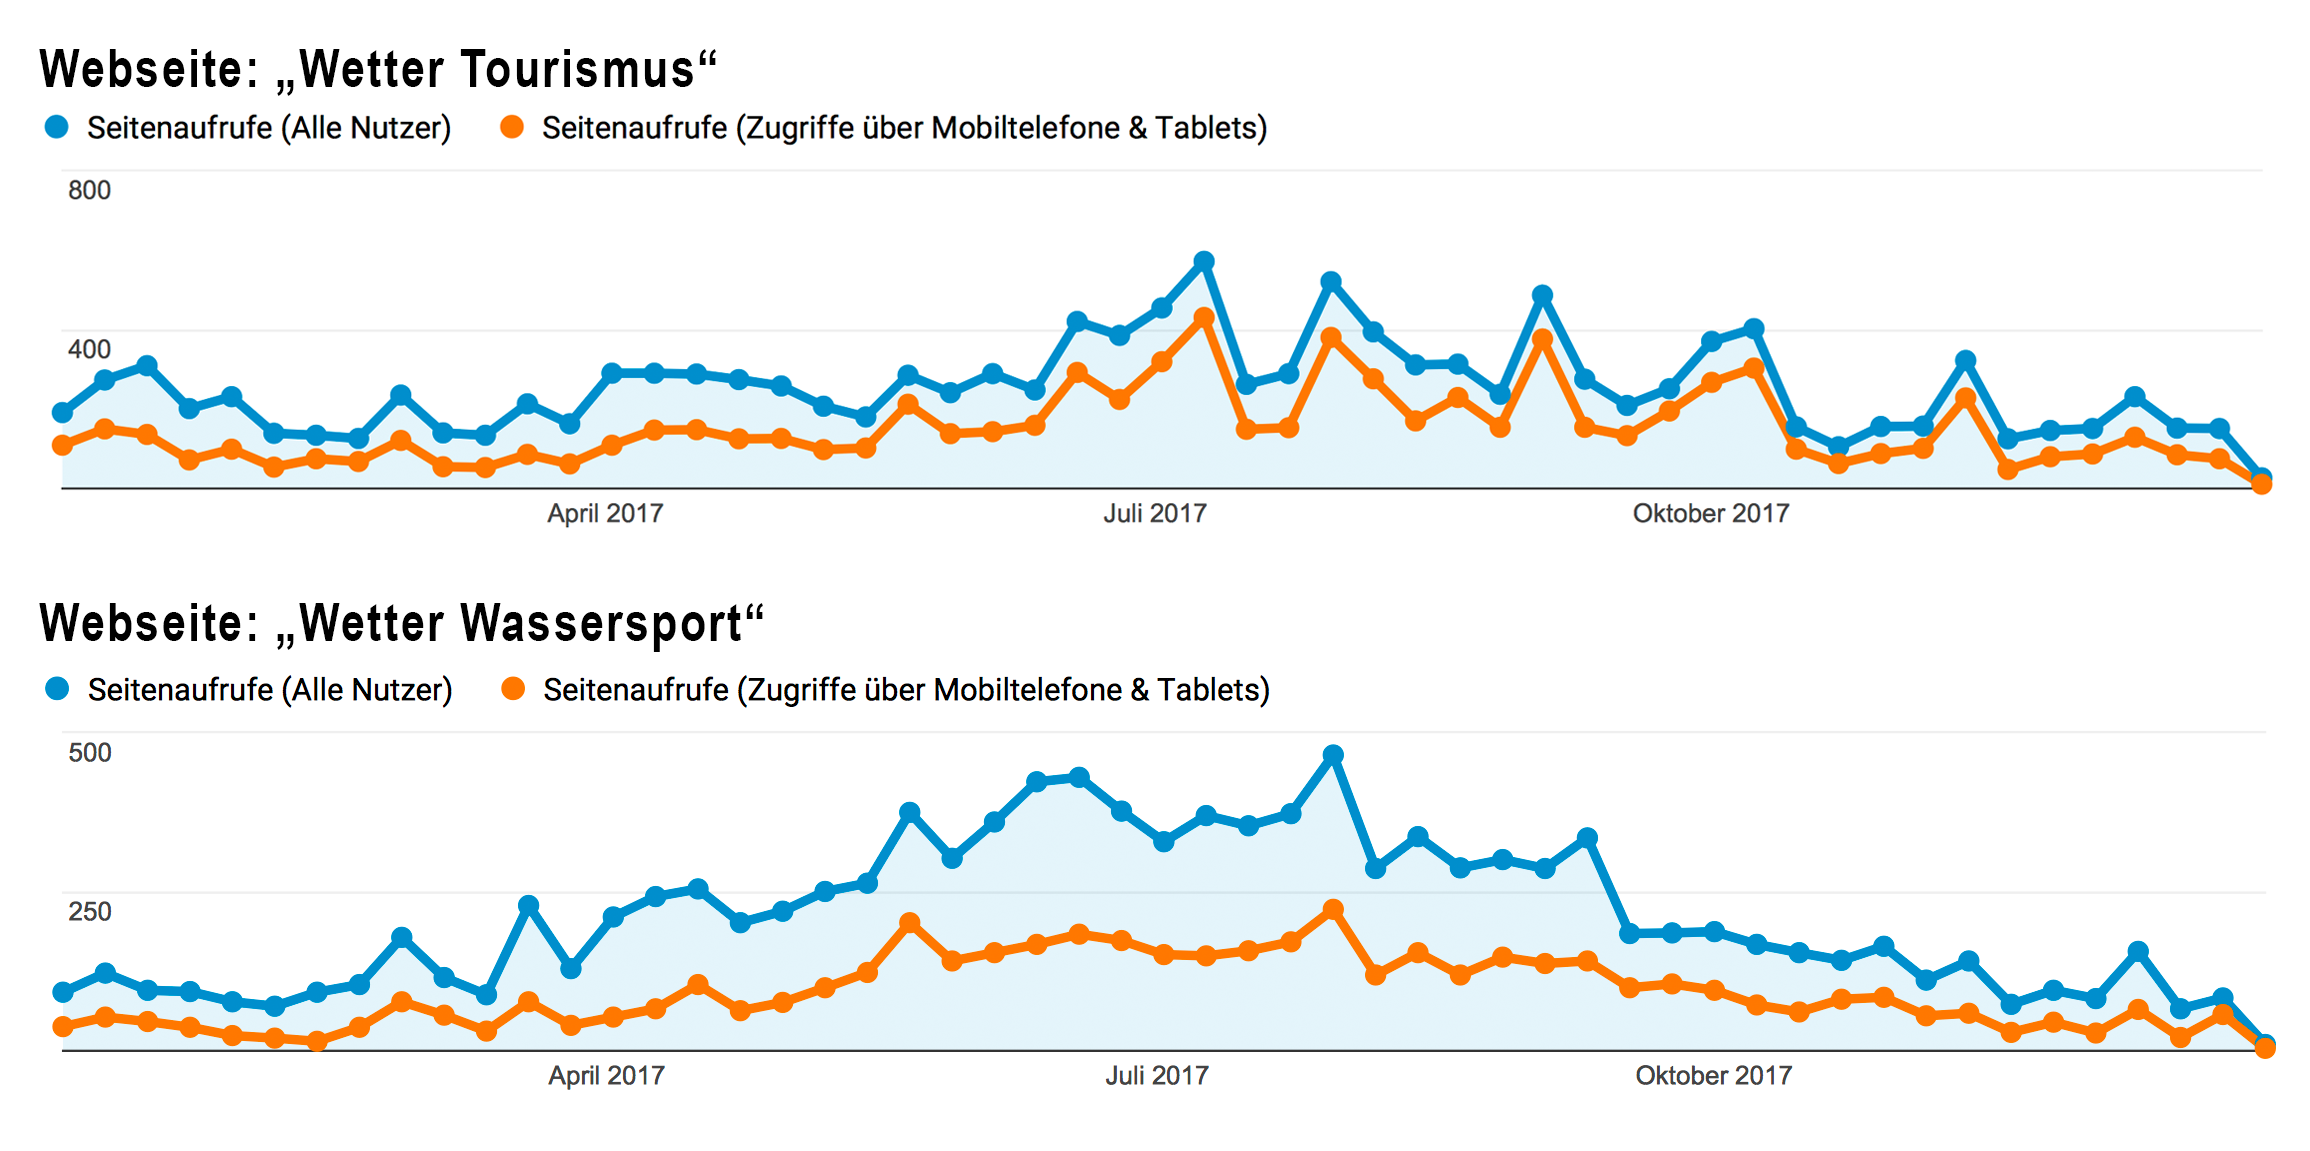
\includegraphics[width=\textwidth-2\fboxsep-2\fboxrule]{img/google_mobile}}
	\centering
	\caption{Anteil der mobilen Zugriffe auf die Wetterwebseite}
	\label{img:google_mobile}
\end{figure}

\noindent
Die Auswertung von Google Analytics, wie in Abbildung\,\ref{img:google_browser} dargestellt, zeigt zudem, dass mehr als zwei Drittel der Zugriffe über den Safari- beziehungsweise Chrome-Browser erfolgen und dass die Webcam die mit Abstand beliebteste Funktion der Wetterstation ist.

\begin{figure}[htb!]
	\centering
	\fbox{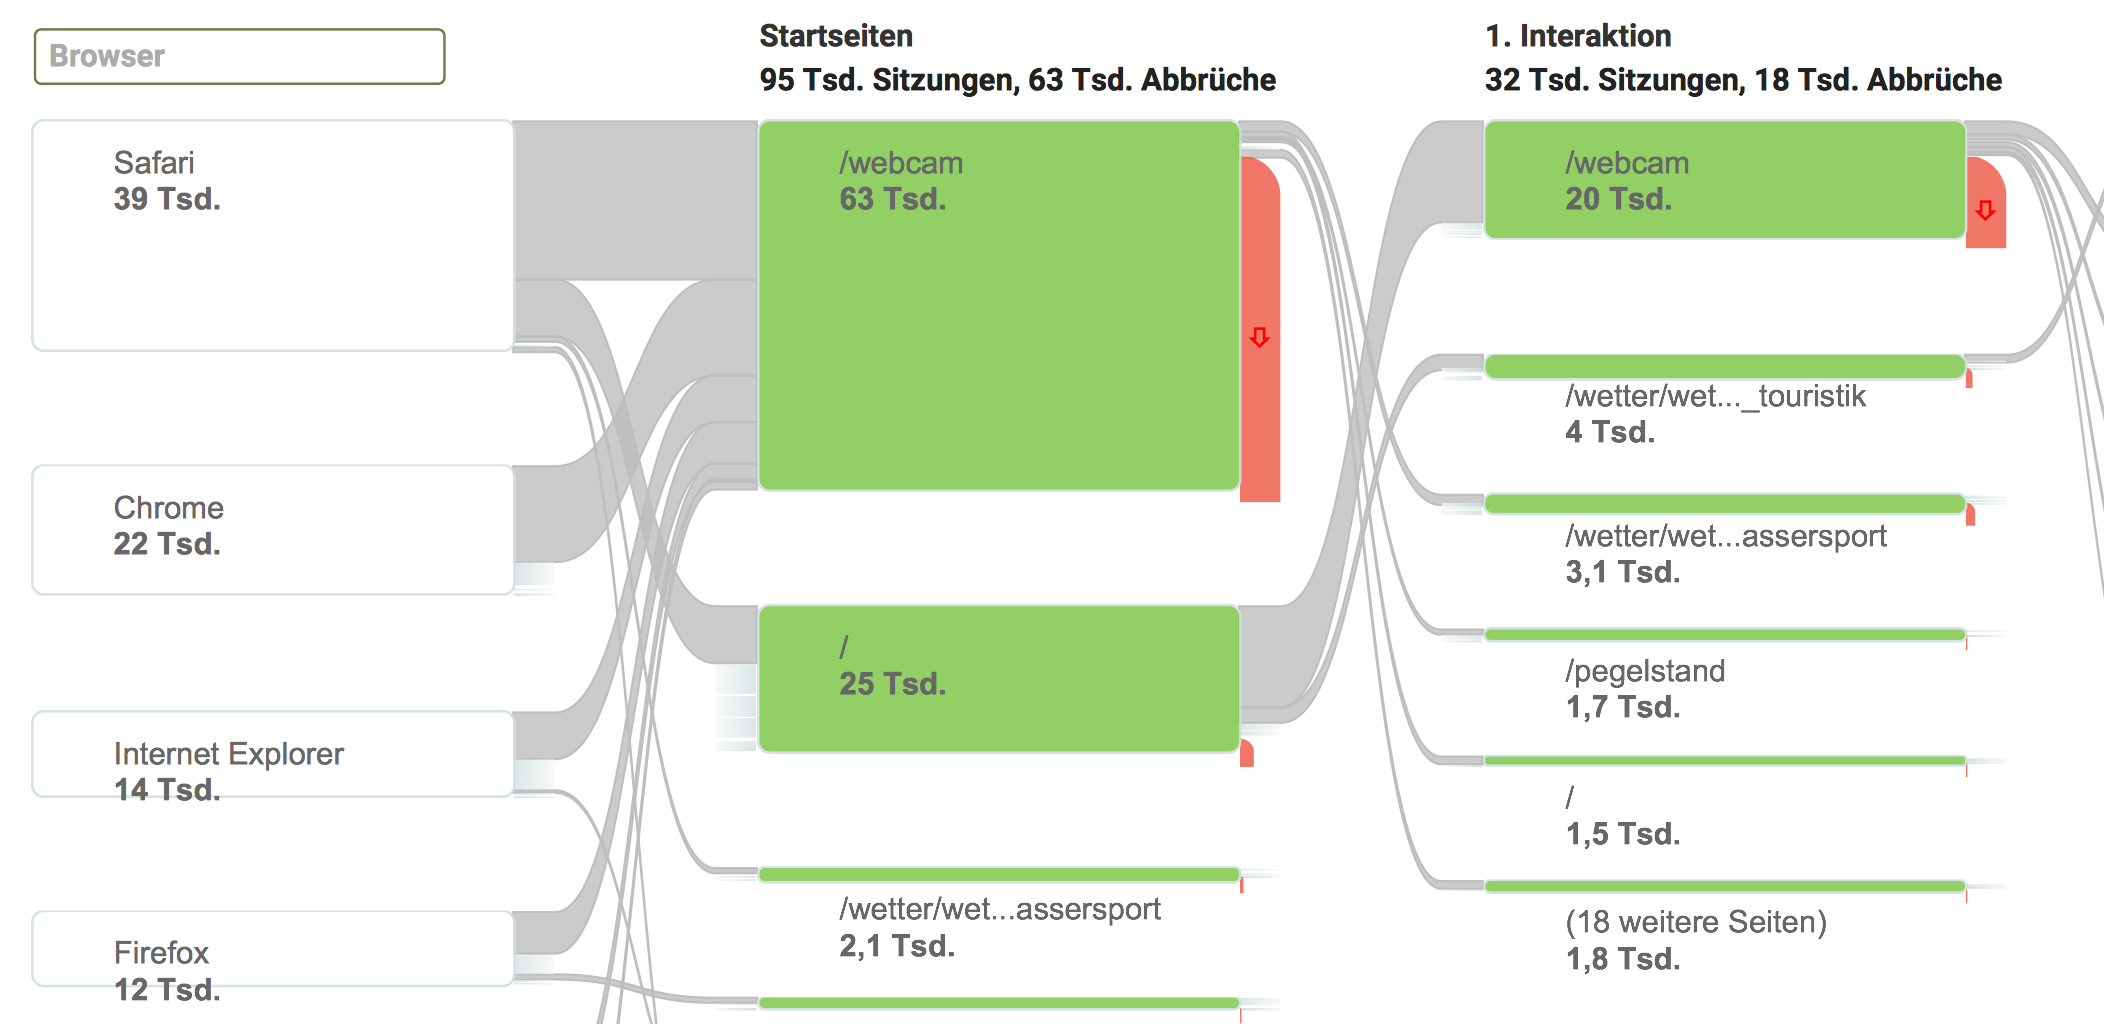
\includegraphics[width=\textwidth-2\fboxsep-2\fboxrule]{img/google_browser}}
	\caption{Verwendete Browser und Beliebtheit der Seiten}
	\label{img:google_browser}
\end{figure}



%% ############################################################################
%% Unterkapitel
%% ############################################################################
\subsection{Konzeption der crossplattformfähigen Benutzeroberfläche}
Wie im Abschnitt\,\ref{subsec:googleAnalytics} aufgezeigt, werden bereits heute 50\,\% bis 80\,\% der Website-Aufrufe von mobilen Geräten ausgeführt, Tendenz steigend. Es ist deshalb naheliegend, das mobile Design als Ausgangspunkt der Entwicklung zu verwenden. Diese Vorgehensweise nennt sich \emph{Mobile First}. Es ist ein Designkonzept, das von Luke Wroblewski 2009 das erste Mal vorgeschlagen wurde. Die \href{https://www.w3.org/TR/mobile-bp}{\emph{ Mobile Web Best Practices}} des \emph{W3C}\footnote{W3C: World Wide Web Consortium} empfiehlt zudem, dass sämtliche Informationen, die in der Desktop-Version zur Verfügung stehen, auch von der mobilen Seite aufgerufen werden können. Dieser Grundsatz nennt sich \emph{One Web Design}.

\begin{figure}[htb!]
  \fbox{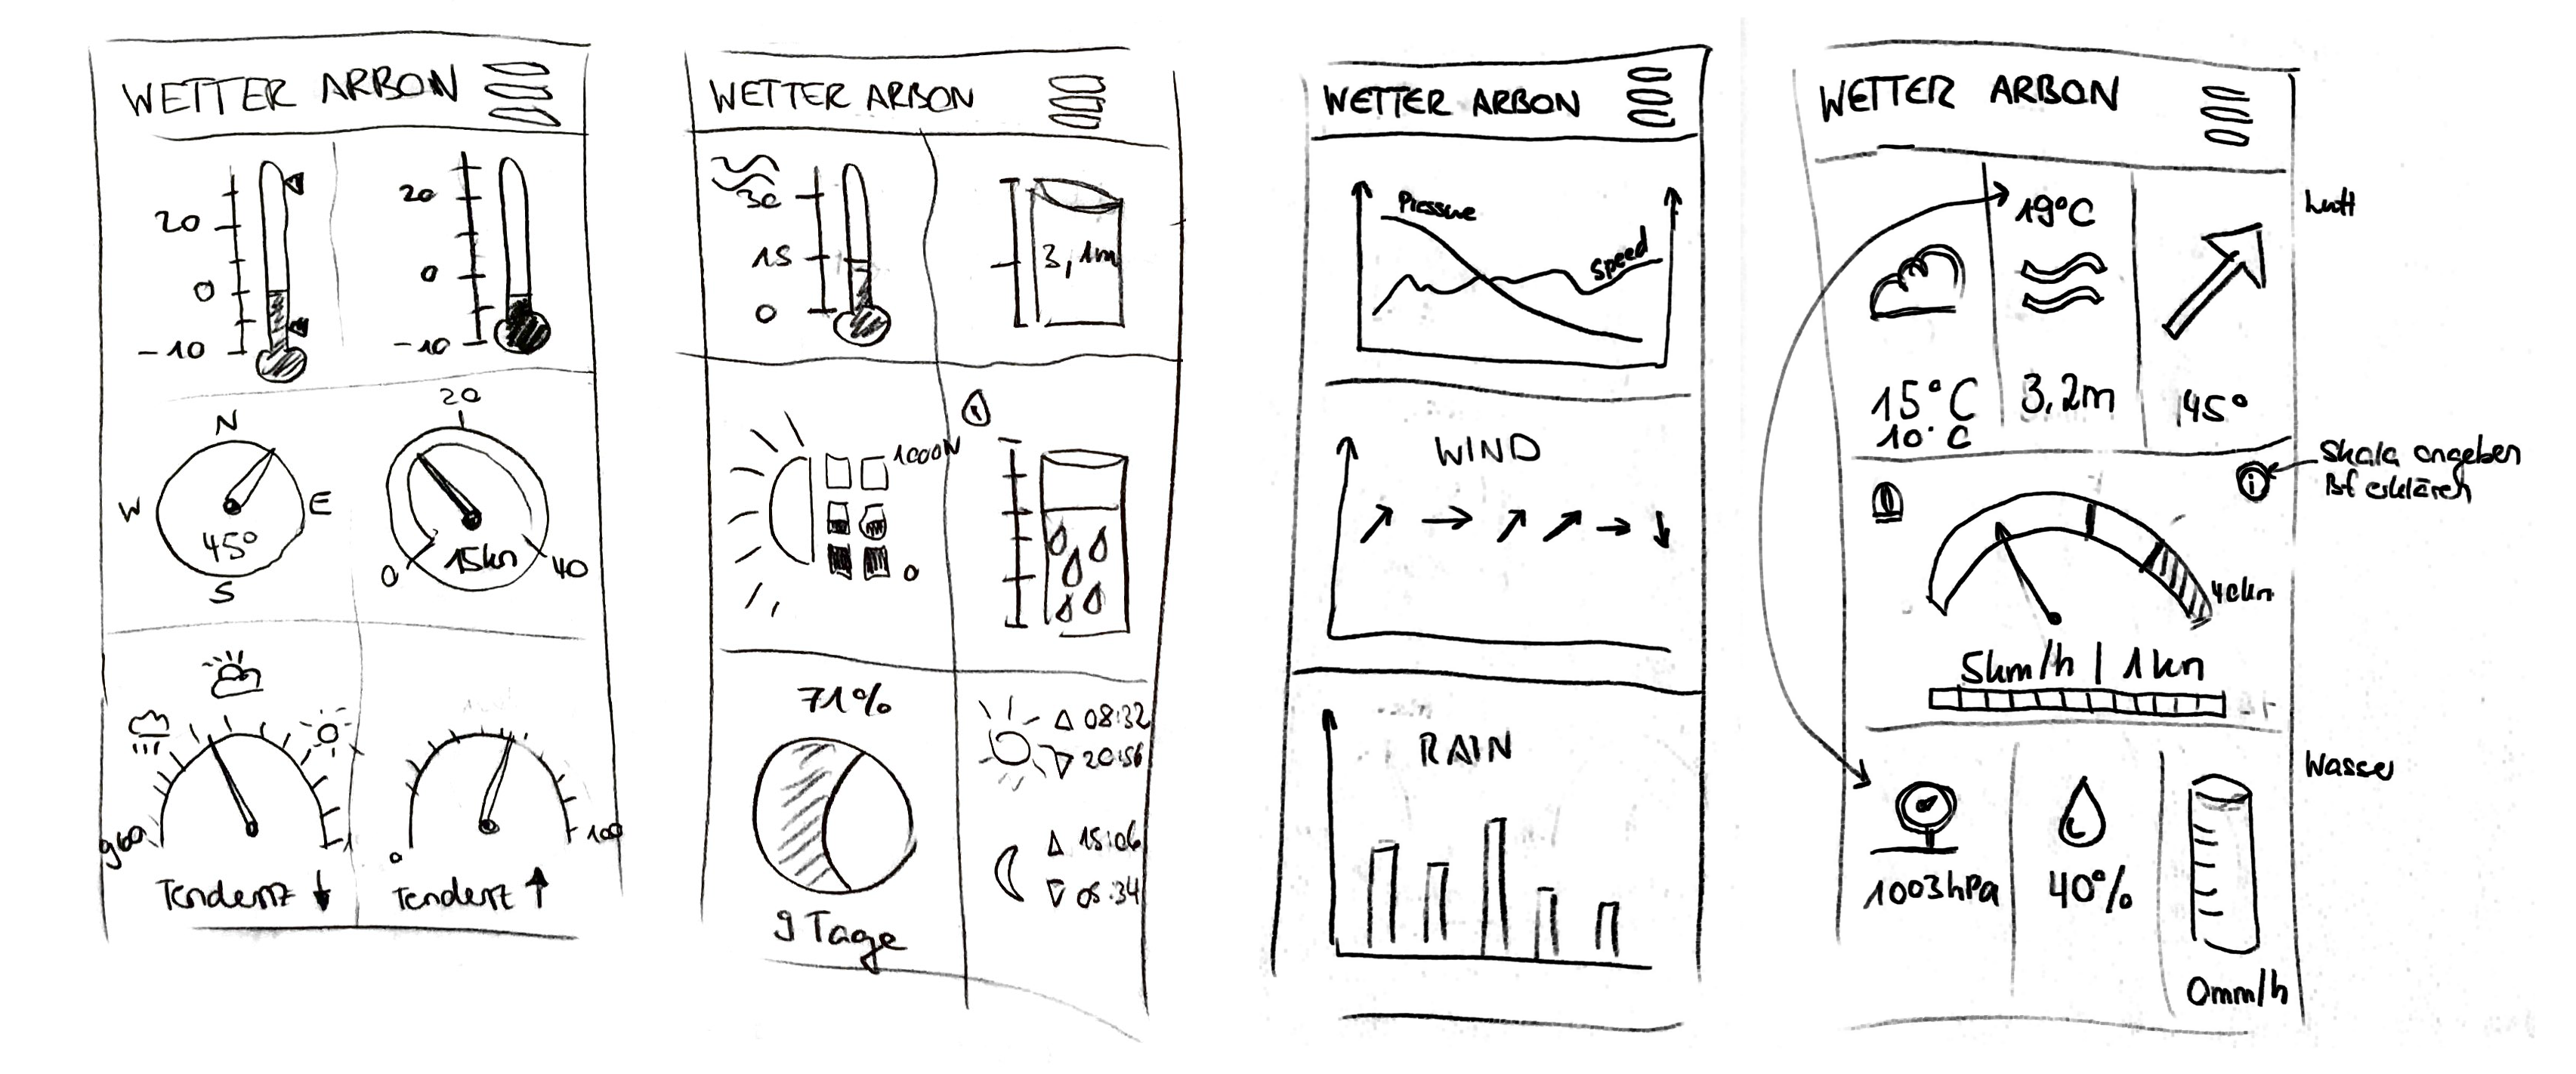
\includegraphics[width=\textwidth-2\fboxsep-2\fboxrule]{img/scribbles}}
	\centering
	\caption{Erste Designentwürfe nach dem Mobile First Prinzip}
	\label{img:scribbles}
\end{figure}


\noindent
Beim Erstellen der ersten Designentwürfe (vgl. Abbildung \ref{img:scribbles}) zeigte sich, dass die einfachste Möglichkeit, die Daten auf allen Bildschirmgrössen darzustellen, darin besteht, die Informationen in kleine logische Blöcke zu unterteilen. Diese Blöcke können dann je nach Bildschirmgrösse verschieden angeordnet werden. Dieses Kachel-Design ist eine gängiges Prinzip, um das Gestaltungsgesetz der Zusammengehörigkeit umzusetzen und eignet sich hervorragend für das responsive Grid-Design, welches im Abschnitt \ref{subsec:responsiveFactors} erklärt wird.


\subsubsection{Auswahl der CSS-Bibliothek}
Sämtliche Artefakte sollen möglichst einfach gehalten werden. Für die Gestaltung der Benutzeroberfläche wurde beschlossen, eine CSS-Bibliothek zu verwenden. Es wurden drei verschiedene CSS-Bibliotheken evaluiert und mittels Nutzwertanalyse bewertet. Das Resultat ist in Tabelle\,\ref{table:css-bibliothek} ersichtlich. Die Erklärungen dazu sind im Anschluss daran aufgelistet.

% Nutzwertanalyse
\begin{table}[htbp!]
  \setlength\extrarowheight{3pt} % for a more "open" look
  \begin{tabularx}{\textwidth}{|>{\RaggedRight\hspace{0pt}}p{3.5cm}|p{2.5cm}||X|X|X|X|}

  \hline
  & \bfseries Gewichtung
  & \bfseries \href{https://www.w3schools.com/w3css/default.asp}{W3.css}
  & \bfseries \href{https://purecss.io/start/}{Pure.css}
  & \bfseries \href{http://getbootstrap.com/docs/4.1/getting-started/introduction/}{Bootstrap} \\

  \hline
  \textbf{Grid Design}
  & 4
  & 2
  & 3
  & 3 \\

  \hline
  \textbf{Card-Design}
  & 3
  & 3
  & 1
  & 3 \\

  \hline
  \textbf{Dokumentation}
  & 3
  & 3
  & 2
  & 2 \\

  \hline
  \textbf{Footprint}
  & 2
  & 3
  & 3
  & 1 \\

  \hline
  \textbf{Funktionsumfang}
  & 1
  & 3
  & 2
  & 2 \\

  \hline
  \hline
  \textbf{Total}
  & -
  & 14
  & 11
  & 11 \\

  \hline
  \textbf{gewichtet}
  & -
  & 35
  & 29
  & 31 \\

  \hline
  \end{tabularx}
  \caption{Nutzwertanalyse der evaluierten CSS-Bibliotheken}
  \label{table:css-bibliothek} % label muss NACH caption stehen!!!!
\end{table}


\paragraph*{Kriterien für die Auswahl}
Folgende Kriterien für die Auswahl der CSS-Bibliothek wurden berücksichtigt:
\begin{itemize*}
\item Grid Design: Unterstützt die Bibliothek das Grid Design und mehrere Displaygrössen, um responsive Webseiten zu gestalten?
\item Card Design: Unterstützt die Bibliothek das Card Design?
\item Dokumentation und Usabilty: Sind die Funktionen zentral und verständlich dokumentiert und ist eine Suchfunktion vorhanden?
\item Footprint: Die CSS-Bibliothek wird auf Mobilgeräte heruntergeladen und sollte deshalb nicht allzu gross sein
\item Funktionsumfang: Sind sämtliche benötigten Funktionen vorhanden oder müssen Zusatzbibliotheken eingebunden werden?
\end{itemize*}


\paragraph*{Gewichtung der Kriterien}
Die Gewichtungsskala für die Kriterien reicht von 1 (weniger wichtig) bis 4 (sehr wichtig). Für die Auswahl der CSS-Bibliothek wurde folgende Gewichtung vorgenommen:
\begin{itemize*}
\item 4 Grid Design: nötig zum Erstellen von modernen responsiven Webseiten
\item 3 Card Design: erhöht die Wahrnehmung der Zusammengehörigkeit
\item 3 Dokumentation: vereinfacht Erstellung und Anpassung
\item 2 Footprint: Bandbreite ist heutzutage nicht mehr so kritisch
\item 1 Funktionsumfang: es werden keine Spezialfunktionen benötigt
\end{itemize*}


\paragraph*{Bewertungsskala für die Kriterien}
Als mögliche Werte für die genannten Kriterien werden die Zahlen 1 (schlecht) bis 3 (gut) verwendet. Im Folgenden wird festgelegt, wann welcher Wert bei den einzelnen Kriterien vergeben wird.
\begin{itemize*}
\item Grid Design
  \begin{enumerate*}
  \item keine Unterstützung bzw. weniger als 3 Displaygrössen
  \item volle Unterstützung, min. 3 Displaygrössen
  \item volle Unterstützung, min. 4 Displaygrössen
  \end{enumerate*}
\item Card Design
  \begin{enumerate*}
  \item keine Unterstützung
  \item kein Card Design, aber ähnliches Prinzip
  \item volle Unterstützung
  \end{enumerate*}
\item Dokumentation und Usabilty
  \begin{enumerate*}
  \item Keine zentrale Dokumentation vorhanden
  \item Zentrale Dokumentation vorhanden, unübersichtlich, keine Suchfunktion
  \item Zentrale Dokumentation vorhanden, ausführlich und verständlich
  \end{enumerate*}
\item Footprint
  \begin{enumerate*}
  \item Grösser als 100kB
  \item Zwischen 50kB und 100kB
  \item Kleiner als 50kB
  \end{enumerate*}
\item Funktionsumfang
  \begin{enumerate*}
  \item nicht alle nötigen Funktionen vorhanden
  \item Sämtliche nötigen Funktionen vorhanden, mehrere Dateien
  \item Sämtliche nötigen Funktionen vorhanden, eine Datei
  \end{enumerate*}
\end{itemize*}


\paragraph*{Entscheidung}
Als Sieger stellt sich die W3.css-Bibliothek heraus, da sie mit Ausnahme der Beschränkung auf 3\,Displaygrössen alle Kriterien vollständig erfüllt.


\subsubsection{Responsive Webdesign}
\label{subsec:responsiveFactors}
Beim \emph{Responsive Webdesign} passt sich die Benutzeroberfläche automatisch der Bildschirmgrösse des Endgeräts an. Die Idee des Responsive Webdesigns wurde 2010 von Ethan Marcotte in einem Artikel des Magazins \emph{A List Apart}~\cite{EthMarRWD} veröffentlicht. Hintergrund war, dass man nicht für jedes neue Gerät eine eigene Webseite erstellen wollte. Marcotte schreibt von drei Faktoren, die ein responsive Webdesign voraussetzt: \emph{fluid grids}, \emph{flexible images} und \emph{media queries}. Fluid grids bedeutet, dass sich die Anordnung der Elemente dynamisch der Bildschirmgrösse anpasst. Flexible images haben keine feste Grösse, sondern nutzen den ihnen zu Verfügung stehenden Platz optimal aus und die media queries sind die technische Basis. Im Folgenden wird das Konzept der fluid grids genauer erklärt.

\begin{figure}[htb!]
  \fbox{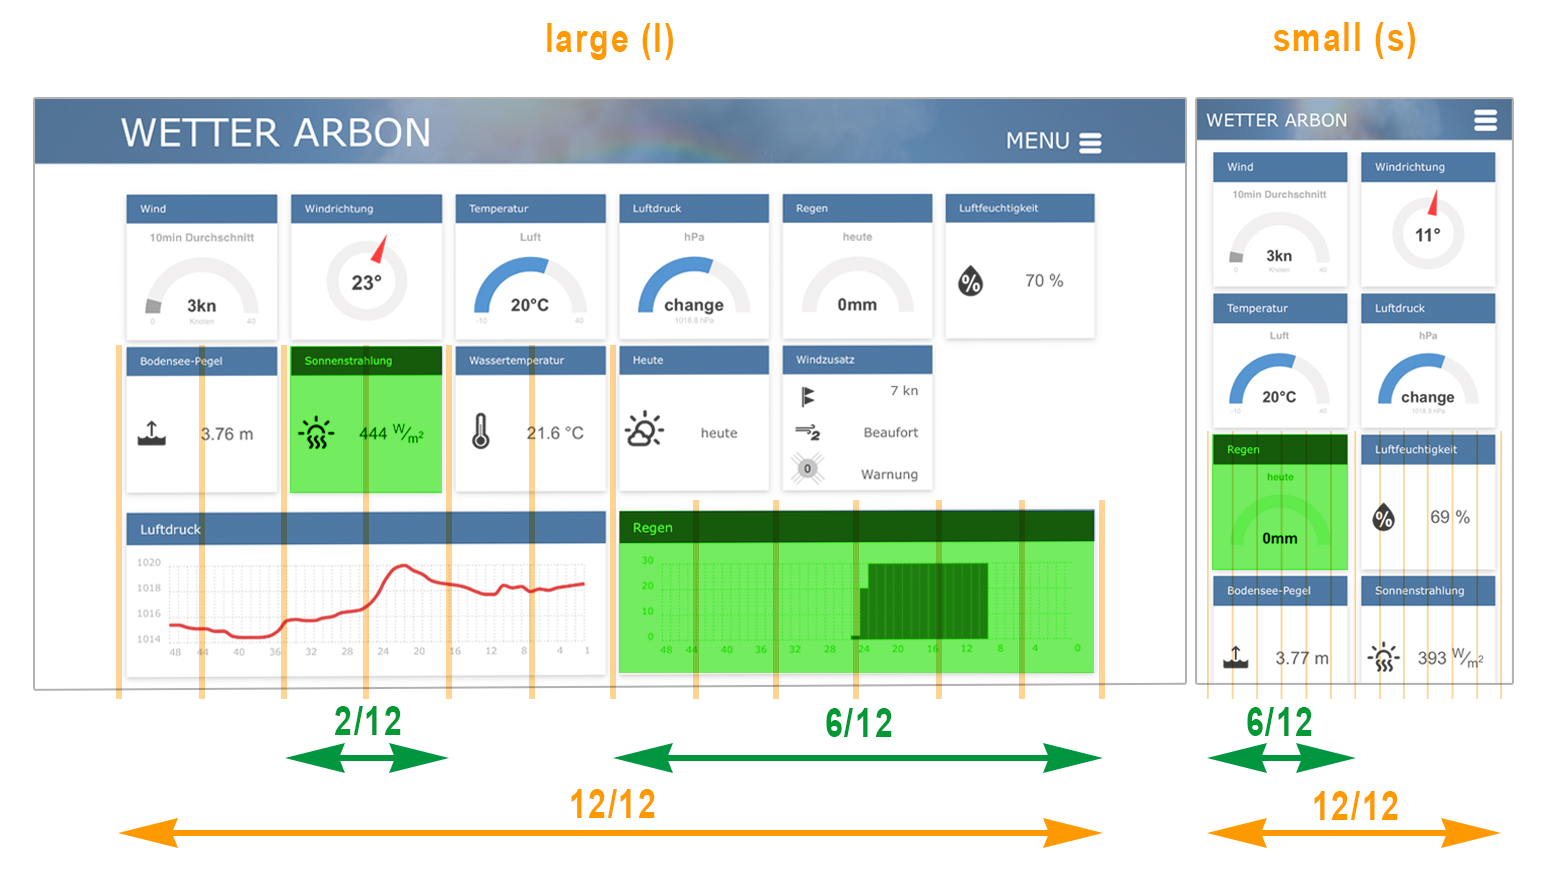
\includegraphics[width=\textwidth-2\fboxsep-2\fboxrule]{img/kacheln2}}
	\centering
	\caption{Anordnung der Kacheln auf grossen und kleinen Bildschirmen}
	\label{img:kacheln2}
\end{figure}

\noindent
Das Grid-System vereinfacht das Erstellen von responsiven Webseiten, indem es den Bildschirm beziehungsweise den zur Verfügung stehenden Platz unabhängig von dessen Grösse in mehrere gleich breite Spalten einteilt (siehe orange Markierung in Abbildung\,\ref{img:kacheln2}). Die Anzahl Spalten ist frei wählbar bzw. abhängig von der gewählten CSS-Bibliothek (bei w3.css sind es 12 Spalten). Über eine media query fragt die Webseite beziehungsweise der Browser die Grösse des Bildschirms in Pixel ab und bestimmt dann, wie viele Spalten breit ein Element sein soll (grüne Markierung in Abbildung\,\ref{img:kacheln2}). Die gleiche Kachel ist also auf einem grossen Bildschirm  \nicefrac{2}{12} breit und auf einem kleinen Bildschirm \nicefrac{6}{12}. Unter \emph{w3.css} sind drei Bildschirmgrössen vorgesehen (small, medium und large). Die Grenzen sind folgendermassen festgelegt:

\begin{description*}
  \item [Small:] s $\leq$ 600px (z.B. iPhone Hochformat)
  \item [Medium:] 600px < m $\leq$ 992px (z.B. iPhone Querformat, iPad Hochformat)
  \item [Large]: l > 992px (z.B. Desktop)
\end{description*}

\noindent
Den Kacheln kann nun über die Klasse (z.B. l2 m3 s6) jeweils ein bestimmtes Verhalten bei den drei Bildschirmgrössen vorgeschrieben werden. Die Kacheln mit den aktuellen Wetterdaten sind zum Beispiel auf grossen (large) Bildschirmen \nicefrac{2}{12}, auf mittleren Bildschirmen \nicefrac{3}{12} und auf kleinen Bildschirmen \nicefrac{6}{12} breit. Bei der Darstellung der Wetterdatenverläufe werden bei mittleren und grossen Bildschirmen zwei nebeneinander dargestellt (\nicefrac{6}{12}) und bei kleinen Bildschirmen alle untereinander (\nicefrac{12}{12} ), wie in Listing\,\ref{lst:kacheln} ersichtlich.

\vspace{3mm}
\begin{lstlisting}[label=lst:kacheln,caption=Konfiguration der Anzahl Kacheln abhängig von der Bildschirmgrösse, language=HTML5, style=htmlcssjs]
<!-- Aktuelle Daten -->
<div class="l2 m3 s6">...</div>
<!-- Datenverlauf -->
<div class="l6 m6 s12">...</div>
\end{lstlisting}
\vspace{3mm}

%% ############################################################################
%% Unterkapitel
%% ############################################################################
\subsection{Grafische Darstellung der aktuellen Wetterdaten}
Die Anzeigeelemente für die aktuellen Messwerte sollen ebenfalls mit Hilfe einer Bibliothek erstellt werden. Damit die Grafiken optimal mit dem responsiven Webdesign zusammenspielen, müssen sie ein flexibles Layout aufweisen, das heisst ihre Grösse dem vorhandenen Platz anpassen. Dies nicht nur beim Aufrufen der Seite, sondern auch beim Ändern der Fenstergrösse. Zudem muss es einfach möglich sein, die Werte zu aktualisieren.

\begin{figure}[h!]
  \fbox{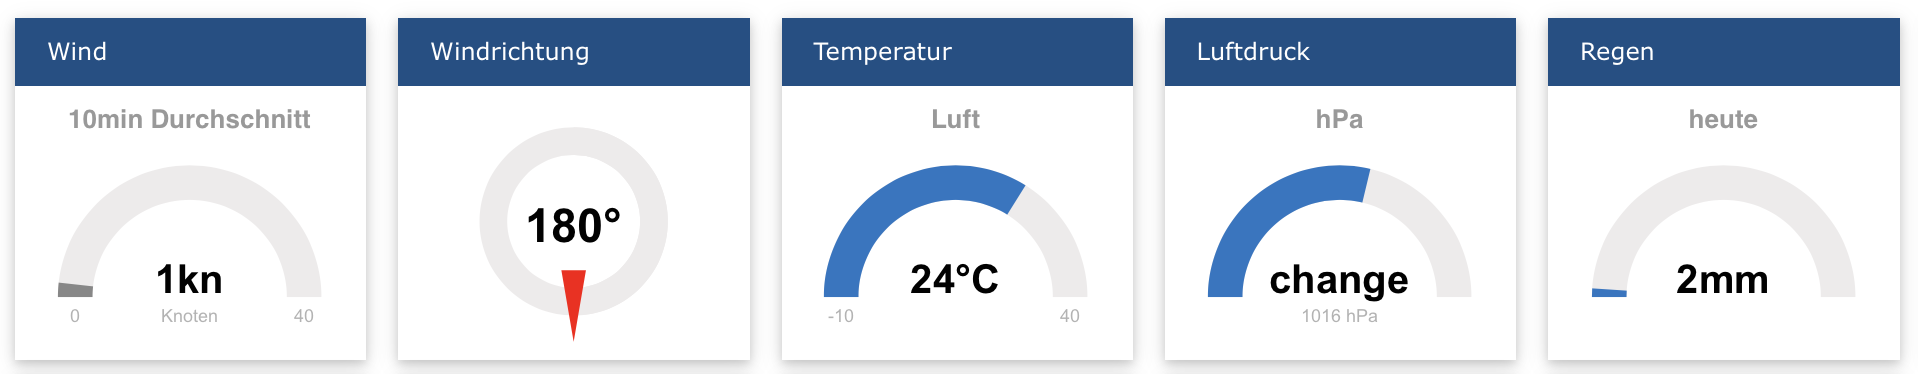
\includegraphics[width=\textwidth-2\fboxsep-2\fboxrule]{img/gauges}}
	\centering
	\caption{Anzeigelemente mit JustGage/Raphaël}
	\label{img:gauges}
\end{figure}

\noindent
Die Anzeige sollte möglichst ein klares Design aufweisen, aber trotzdem individuell anpassbar sein. Eine sehr einfache Javascript-Bibliothek, die diese Anforderungen erfüllt, ist \emph{JustGage}\footnote{ \url{http://justgage.com}}. Die Grafiken lassen sich über eine Javascript-Datei konfigurieren, sind im vektorbasierten svg-Format und dadurch von praktisch allen Browsern darstellbar. JustGage basiert auf der \textit{Raphaël}\footnote{ \url{http://dmitrybaranovskiy.github.io/raphael/}} Javascript-Bibliothek.

\noindent
Die Konfiguration eines Anzeigelements (Gauge) ist in Listing\,\ref{lst:gaugeJS} beispielhaft dargestellt. Jedes Element besitzt eine \emph{id} und einen Wert (\emph{value}) sowie optionale Angaben wie Skalaanfangs- und Endwerte und Beschriftungszusätze.

\vspace{3mm}
\begin{lstlisting}[label=lst:gaugeJS,caption=Konfiguration einer Gauge in Javascript, language=JavaScript, mathescape, style=htmlcssjs]
var temperature_gauge = new JustGage({
  id:     'temperature_gauge',
  value:  initialValues.v1.data.temperature.value,
  min:    -10,
  max:     40,
  symbol: ${^\circ}$C,
  title:  'Luft'
});
\end{lstlisting}
\vspace{3mm}

\noindent
Um die Grafik anzuzeigen, muss nur ein \emph{div} mit derselben \emph{id} auf der Webseite erstellt werden, wie in Listing \ref{lst:gaugeHTML} dargestellt.

\vspace{3mm}
\begin{lstlisting}[label=lst:gaugeHTML,caption=Container für die Gauge auf der Webseite, language=HTML5, style=htmlcssjs]
<!-- Lufttemperatur -->
<div class="l2 m3 s6">
    <div><p>Temperatur</p></div>
    <div id="temperature_gauge" class="gauge"></div>
</div>
\end{lstlisting}
\vspace{3mm}


\noindent
Messwerte ohne Relation zu einem Maximalwert sind nicht als Gauge, sondern als einfacher Text dargestellt (siehe Abbildung\,\ref{img:icons}). Die Messgrösse wird dabei einerseits im Titel der Kachel angegeben, und andererseits grafisch als Symbol neben dem Messwert. Dazu wurde eine Icon-Bibliothek gewählt, die möglichst alle benötigen Icons enthält, kostenlos ist, und deren Grafiken im svg-Format vorliegen. Als geeignet schienen die \emph{Weather Icons} von Erik Flowers\footnote{ \url{http://erikflowers.github.io/weather-icons/}} .

% Die Messwerte sind einerseits über den Titel beschrieben, sie enthalten aber zusätzlich ein passendes Icons.

\vspace{3mm}
\begin{figure}[htb!]
  \fbox{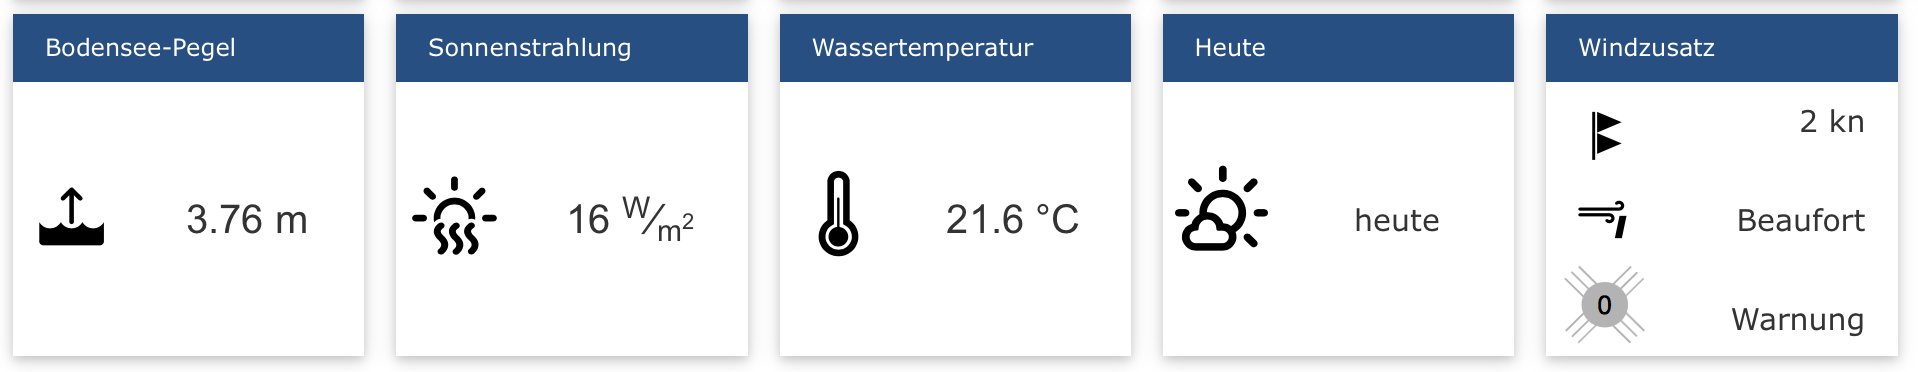
\includegraphics[width=\textwidth-2\fboxsep-2\fboxrule]{img/icons}}
	\centering
	\caption{Ausgewählte Icons aus der Weather Icons Bibliothek}
	\label{img:icons}
\end{figure}



%% ############################################################################
%% Unterkapitel
%% ############################################################################
\subsection{Grafische Darstellung der Wetterdatenverläufe}
Die Wetterverlaufsdarstellung liefert einen Überblick über das Wettergeschehen der letzten beiden Tage, wie beispielhaft in Abbildung\,\ref{img:charts} dargestellt ist. Im Folgenden wird erläutert, welche Javascript-Bibliothek dafür ausgewählt wurde und wie die unterschiedlichen Messverläufe dargestellt werden.

% Die Samplerate beträgt 1h, d.h. die Daten werden aus der Tabelle der historischen Werte abgerufen.
% in diesem Kapitel: Auswahl JS-Bibliothek, y-Achse, Windrichtung, Windvergleich

\begin{figure}[h!]
  \fbox{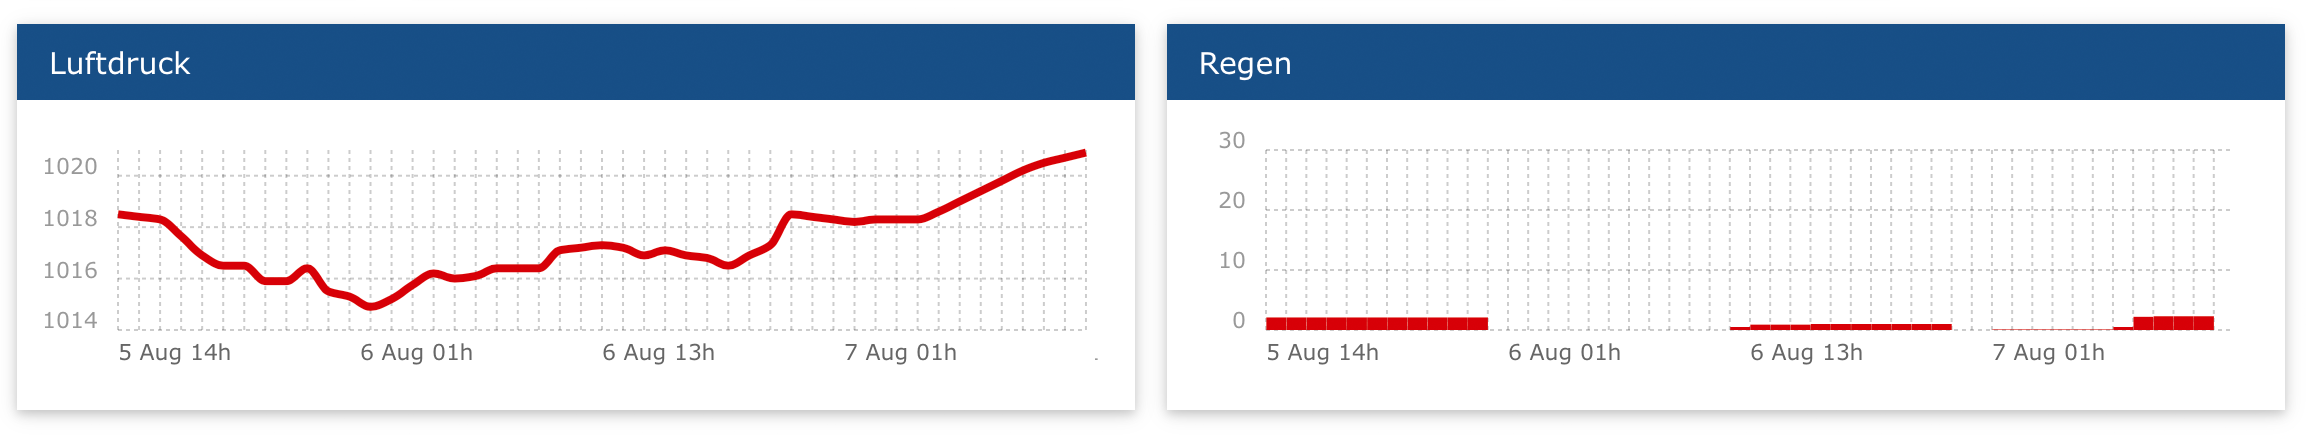
\includegraphics[width=\textwidth-2\fboxsep-2\fboxrule]{img/charts}}
	\centering
	\caption{Darstellung der Messverläufe mittels Linien- und Balkendiagrammen}
	\label{img:charts}
\end{figure}


\subsubsection{Auswahl der Javascript-Bibliothek}
Für die Darstellung der Messwertverläufe wurde ebenfalls auf eine Bibliothek zurückgegriffen. Als Erstes wurden Javascript-Bibliotheken gesucht, die ein ansprechendes Design aufweisen. Übrig geblieben sind die drei Javascript-Bibliotheken: \emph{chartist}, \emph{Fusion Charts} und \emph{Google Charts}. \emph{D3} ist zwar \emph{DIE} Javascript-Bibliothek, wenn es um Visualisierungen im Web geht, hat aber keine vorgefertigten Diagramme und benötigt entsprechend viel Aufwand und Einarbeitungszeit, weshalb sie nicht berücksichtigt wurde. Die drei potentiellen Javascript-Bibliotheken wurden mittels Nutzwertanalyse einander gegenübergestellt. Das Resultat ist in Tabelle\,\ref{table:js-framework} aufgeführt. Die Auswahl und Gewichtung der Kriterien ist im Anschluss daran erklärt.

% Nutzwertanalyse
\vspace{3mm}
\begin{table}[htbp!]
  \setlength\extrarowheight{3pt} % for a more "open" look
  \begin{tabularx}{\textwidth}{|>{\RaggedRight\hspace{0pt}}p{3.5cm}|p{2.5cm}||X|X|X|X|}

  \hline
  & \bfseries Gewichtung
  & \bfseries \href{https://gionkunz.github.io/chartist-js/index.html}{chartist.js}
  & \bfseries \href{https://www.fusioncharts.com}{Fusion Charts}
  & \bfseries \href{https://developers.google.com/chart/}{Google Charts}\\

  \hline
  \textbf{Footprint}
  & 1
  & 3
  & 1
  & 2 \\

  \hline
  \textbf{Barrierefrei}
  & 2
  & 2
  & 2
  & 1 \\
  \hline
  \textbf{Anpassbarkeit}
  & 4
  & 2
  & 3
  & 2 \\

  \hline
  \textbf{Dokumentation}
  & 3
  & 3
  & 3
  & 3 \\

  \hline
  \textbf{Funktionsumfang}
  & 4
  & 2
  & 2
  & 2 \\

  \hline
  \hline
  \textbf{Total}
  & -
  & 15
  & 12
  & 13 \\

  \hline
  \textbf{gewichtet}
  & -
  & 44
  & 38
  & 41 \\

  \hline
  \end{tabularx}
  \caption{Nutzwertanalyse der evaluierten Javascript-Bibliotheken}
  \label{table:js-framework} % label muss NACH caption stehen!!!!
\end{table}


\paragraph*{Kriterien für die Auswahl}
Folgende Kriterien für die Auswahl der Javascript-Bibliothek wurden berücksichtigt:
\begin{itemize*}
\item Footprint: Dateigrösse der Bibliothek
\item Barrierefrei: Unterstützung für barrierefreien Zugang vorhanden?
\item Anpassbarkeit: Können die Diagramm auf einfache Weise parametrisiert werden?
\item Dokumentation: Sind die Funktionen zentral und verständlich dokumentiert und ist eine Suchfunktion vorhanden?
\item Kosten: Ist die Bibliothek kostenlos bzw. in einem vertretbaren Rahmen?
\item Funktionsumfang: Werden sämtliche benötigten Diagrammtypen zur Verfügung gestellt?
\end{itemize*}


\paragraph*{Gewichtung der Kriterien}
Die Gewichtungsskala für die Kriterien reicht von 1 (weniger wichtig) bis 4 (sehr wichtig). Für die Auswahl der Javascript-Bibliothek wurde folgende Gewichtung vorgenommen:
\begin{itemize*}
\item 1 Footprint: Heutzutage ist die Dateigrösse nicht mehr so entscheidend
\item 2 Barrierefrei: Ist bei Grafiken nur bedingt möglich
\item 4 Anpassbarkeit: Gewährleistet, dass die Daten wie gewünscht angezeigt werden können
\item 3 Dokumentation: Vereinfacht Erstellung und Anpassung
\item 4 Kosten: Muss erschwinglich sein
\item 4 Funktionsumfang: Möglichst alle Diagrammtypen sollen verfügbar sein
\end{itemize*}


\paragraph*{Bewertungsskala für die Kriterien}
Als mögliche Werte für die genannten Kriterien werden die Zahlen 1 (schlecht) bis 3 (gut) verwendet. Im Folgenden wird festgelegt, wann welcher Wert bei den einzelnen Kriterien vergeben wird.
\begin{itemize*}
\item Footprint
  \begin{enumerate*}
  \item Grösser als 500kB
  \item Zwischen 100kB...500kB
  \item Kleiner als 100kB
  \end{enumerate*}
\item Barrierefrei
  \begin{enumerate*}
  \item keine Unterstützung
  \item teilweise Unterstützung
  \item volle Unterstützung
  \end{enumerate*}
\item Anpassbarkeit
  \begin{enumerate*}
  \item Diagramme sind nur beschränkt anpassbar
  \item Die meisten Parameter sind anpassbar
  \item Alle Parameter sind anpassbar
  \end{enumerate*}
\item Dokumentation
  \begin{enumerate*}
  \item Keine zentrale Dokumentation vorhanden
  \item Zentrale Dokumentation vorhanden, unübersichtlich, keine Suchfunktion
  \item Zentrale Dokumentation vorhanden, ausführlich und verständlich
  \end{enumerate*}
\item Kosten
  \begin{enumerate*}
  \item Mehr als 10CHF/Monat
  \item Maximal 10CHF/Monat
  \item Kostenlos
  \end{enumerate*}
\item Funktionsumfang
  \begin{enumerate*}
  \item Säulen- und Balkendiagramme vorhanden
  \item Interpolation von fehlenden Werten möglich
  \item Pfeildiagramm für Windrichtungsanzeige vorhanden
  \end{enumerate*}
\end{itemize*}


\paragraph*{Entscheidung}
\emph{Chartist.js} stellt den besten Kompromiss zwischen Funktionsumfang, Einfachheit und Dokumentation dar. Insbesondere die Dateigrösse war ausschlaggebend, da die Webseite, wie in Abschnitt \ref{subsec:googleAnalytics} erklärt, häufig auf Mobilgeräten verwendet wird.


\subsubsection{Skalierung der y-Achse}
Zur Verlaufsdarstellung wird primär das Linien- und Balkendiagramm verwendet, wie in Abbildung\,\ref{img:charts} aufgezeigt. Für jede Grafik wurde entschieden, ob eine automatische Y-Achs-Skalierung sinnvoll ist oder nicht. Bei der Windgeschwindigkeit und den Sonnenstrahlungs- und Regenmesswerten wird bewusst eine fixe Skalierung verwendet, damit auf den ersten Blick erkennbar ist, ob der Wert eher hoch oder eher tief ist. Beim Luftdruck und den Temperaturen hingegen ist die Tendenz wichtig, weshalb möglichst die gesamte Höhe des Diagramms genutzt werden soll. Es wird daher eine automatische Y-Achs-Skalierung verwendet. Die Konfiguration erfolgt in einem einfachen Javascript-File, wie in Listing\,\ref{lst:charts}  dargestellt. Unter \emph{options} kann die y-Achse auf die gewünschten Werte fixiert werden.

% Code-Beispiel
\begin{lstlisting}[label=lst:charts,caption=Konfiguration eines Verlaufsdiagramms, language=HTML5, style=htmlcssjs]
//Regen
var Rain = {
	labels: [48,...,1],
	series: [dataRainHistoric]
};
var options = {
low: 0,
high: 30,
};
new Chartist.Bar('#rain-chart', Rain, options);
\end{lstlisting}

\subsubsection{Anzeige des Windrichtungsverlaufs}
Die Anzeige des Windrichtungsverlaufs ist nicht ganz trivial, da sie von 0 bis 360\,Grad geht und ohne Unterbruch wieder zu 0\,Grad. In der Praxis wird dazu häufig die Darstellung von Pfeilen verwendet, wie in Abbildung\,\ref{img:windrichtung} links dargestellt. Es konnte jedoch keine Bibliothek gefunden werden, die diese Darstellungsart als Template zur Verfügung stellt. Für die Anzeige der Windrichtung wird deshalb ein Punktdiagramm, wie in Abbildung\,\ref{img:windrichtung} rechts dargestellt, verwendet. Auf eine Eigenentwicklung wurde bewusst verzichtet, um die Webseite möglichst benutzerfreundlich und wartungsarm zu belassen.

\begin{figure}[htbp!]
	\centering
  \fbox{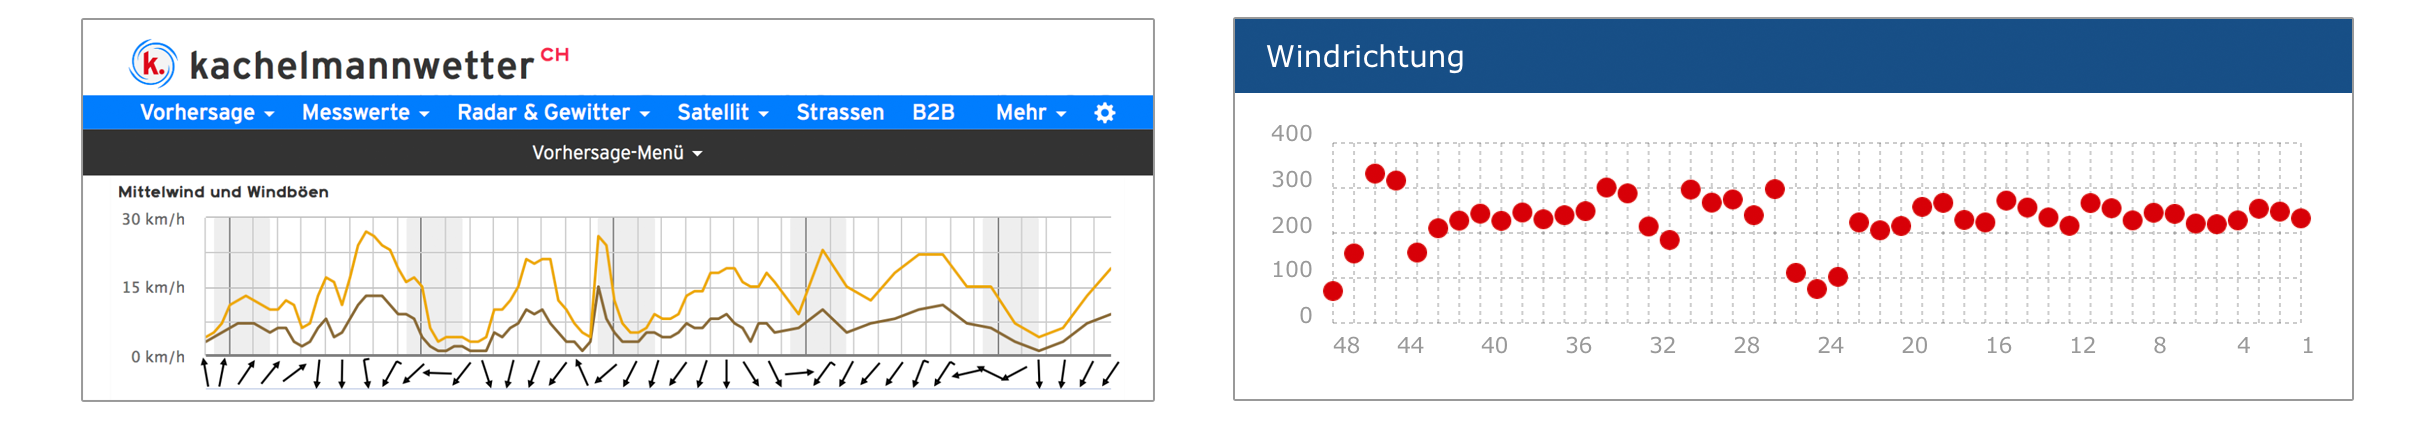
\includegraphics[width=\textwidth-2\fboxsep-2\fboxrule]{img/windrichtung}}
	\caption{Windrichtungsanzeige mittels Pfeilen (links) und Punkten (rechts)}
	\label{img:windrichtung}
\end{figure}

\subsubsection{Vergleich Prognose/Ist-Windgeschwindigkeit}
Insbesondere bei Seglern sind Windprognosedienste sehr beliebt. Sie liefern Windprognosen bis zu fünf Tage voraus. Bei allen Vorhersagediensten ist jedoch rückblickend nicht erkennbar, wie gut die Prognose war. Genau dies ist aber eine spannende Frage, weshalb dieser Vergleich auf der Webseite angezeigt werden soll. Die Messdaten der Wetterstation werden mit zwei kostenlosen Vorhersagediensten verglichen. Dabei wird jeweils die Dreitagesvorschau betrachtet. Für die Windvorhersage wurden folgende zwei Anbieter ausgewählt:
\begin{itemize*}
\item \href{https://openweathermap.org/city/2661731}{Openweathermap}
\item \href{https://www.windfinder.com/forecast/arbon}{Windfinder}
\end{itemize*}

\noindent
Openweathermap ist einer der wenigen Anbieter, welcher eine kostenlose Web-API zur Verfügung stellt und Windfinder ist erfahrungsgemäss unter den Seglern eines der beliebtesten Tools, bietet aber keine API, sondern lediglich ein Widget an (siehe Abbildung\,\ref{img:windfinder} links). Dies Vorhersagedaten müssen aus dem Windfinder-Widget mittels Web-Scrapper extrahiert werden, analog Listing\,\ref{lst:kttgCrawler} auf Seite\,\pageref{lst:kttgCrawler}.

\begin{figure}[h!]
	\centering
  \fbox{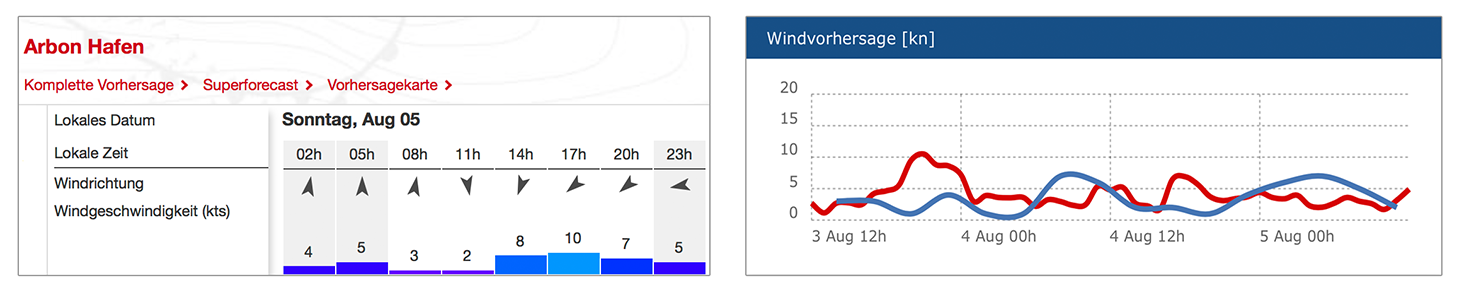
\includegraphics[width=\textwidth-2\fboxsep-2\fboxrule]{img/windfinder}}
	\caption{Widget von Windfinder und Windvergleichsdarstellung}
	\label{img:windfinder}
\end{figure}


Da die Vorhersagedaten nur in die Zukunft angezeigt werden, d.h. wie die Vorhersage von gestern war ist nicht mehr ersichtlich, müssen die Vorhersagedaten abgegriffen und gespeichert werden. Nach den ersten Auswertungen wurde festgestellt, dass die Wettervorhersagedaten von Openweathermap unbrauchbar waren. Sie lagen permanent zwischen 0 und 1 Knoten, auch wenn die Wetterstation 15 Knoten mass. Die Vorhersage von Openweathermap wurde deshalb nicht mehr weiterverfolgt. Das Diagramm des Windvergleichs ist in Abbildung\,\ref{img:windfinder} dargestellt (Vorhersage: blau; Messwert: rot).



%\Diskussionspunkt{- Eintagesvorschau}\newline
%\Diskussionspunkt{- Mittels Tableau? Eigen Webseite?}\newline
%\Diskussionspunkt{- Bild mit Vergleich von Messwerten, Vorhersage Windfinder und Vorhersage Openweathermap}\newline

% Graphen, der den heutigen Tag, links davon die letzten 14 Tage und rechts davon die nächsten drei Tage anzeigt.
% Pro Anbieter und Prognoseart (1Tag bzw. 3 Tage) wird ein eigener Graph erstellt.
% Aus diesen Gründen wird die Webseite zwar veröffentlicht, aber kein Link dazu auf der Webseite zur Verfügung gestellt.
% Werte aus der Stundenwert-Datenbank?

%% ############################################################################
%% Unterkapitel
%% ############################################################################
\subsection{Anzeige der aktuellen Sturmwarn-Situation}
\label{subsec:sturmwarnung}
% was ist der Sturmwarndienst und wie werden die verschiedenen Stufen dargestellt
Auf dem Bodensee gibt es einen Sturmwarndienst, der die Schiffsführer vor aufkommendem Sturm warnen soll. Der Sturmwarndienst wird vom Deutschen Wetterdienst in Zusammenarbeit mit MeteoSchweiz betrieben. Rund um den Bodensee sind dafür über 60 Sturmwarnleuchten installiert (Abbildung \ref{img:sturm2}). Es wird unterschieden zwischen \emph{Starkwindwarnung} und \emph{Sturmwarnung}. Erstere weist auf starke Windböen zwischen 25\,Knoten und 33\,Knoten hin und wird durch Aufleuchten von orangefarbigen Blinklichtern mit ca. 40 orangefarbigen Blitzen pro Minute an den Sturmwarnleuchten signalisiert. Letzere kündigt das Auftreten von Windböen von 34 Knoten und mehr an und wird durch Aufleuchten von orangefarbigen Blinklichtern mit ca. 90 orangefarbigen Blitzen pro Minute an den Sturmwarnleuchten signalisiert~\cite{BSO1976}.

\begin{figure}[htbp!]
	\centering
  \fbox{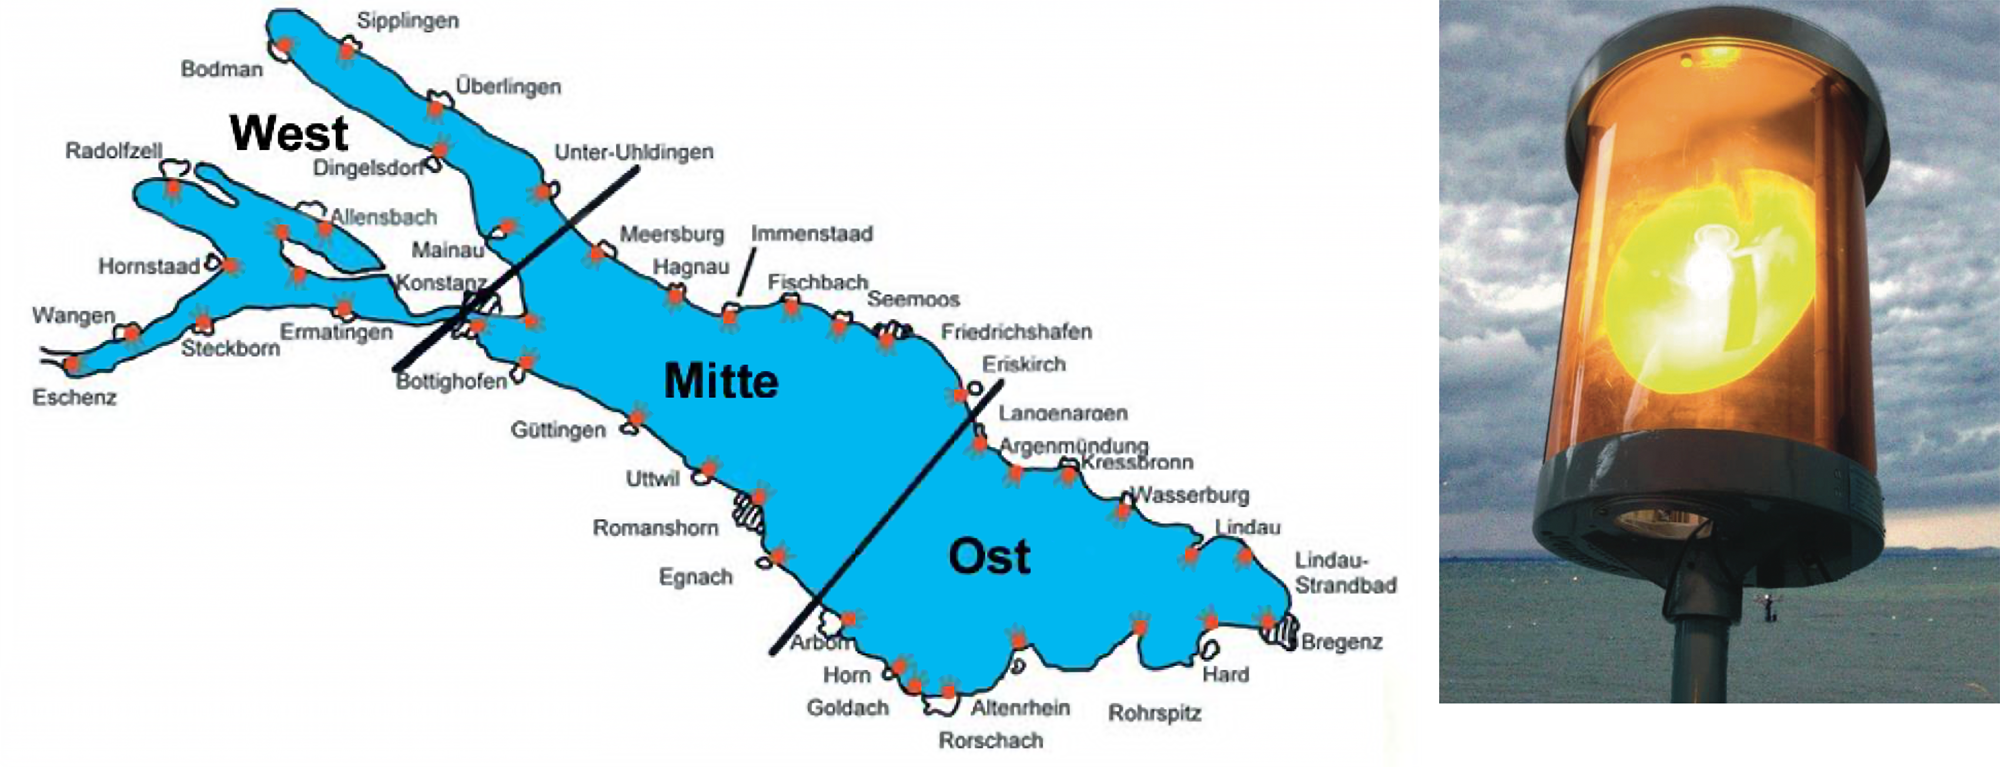
\includegraphics[width=\textwidth-2\fboxsep-2\fboxrule]{img/sturm2}}
	\caption{Warnleuchten des Sturmwarndiensts auf dem Bodensee}
	\label{img:sturm2}
\end{figure}



\subsubsection{Eingeschränkte Bezugsquellen}
% Problem: Kostenpflichtige Informaiton
Der aktuellen Status der Sturmwarnung kann sowohl beim Deutschen Wetterdienst, als auch bei Meteoschweiz kostenpflichtig bezogen werden (ca. 1300CHF/Jahr). Als kostenlose Alternative gibt es nur zwei browserkompatible Quellen: Die eine ist die Warnseite\footnote{ \url{https://www.meteoschweiz.admin.ch/home.html?tab=alarm}}  von Meteoschweiz und die andere die Anzeige auf der Webseite\footnote{ \url{http://www.kttg.ch/kapo/htm/stwarn.shtml}} der Kantonspolizei Thurgau, siehe Abbildung \ref{img:sturmZeit} links. Eine kostenlose API steht nicht zur Verfügung. Meteoschweiz verbietet es zudem, Informationen von ihrer Website abzugreifen. Es wurde deshalb beim Amt für Informatik des Kantons Thurgau, welches die Seite der Kantonspolizei betreut, die Erlaubnis eingeholt, die Sturmwarndaten ihrer Webseite abgreifen zu dürfen (siehe Mail im Anhang\,\ref{anhang:email}) . Beim Vergleich der verschiedenen Quellen wurde festgestellt, dass die Warnleuchten jeweils mit einigen Minuten Verspätung gegenüber der Meldung von Meteoschweiz eingeschaltet werden, siehe Abbildung \ref{img:sturmZeit}. Da der Verzug nicht konstant ist, muss davon ausgegangen werden, dass die Warnleuchten manuell eingeschaltet werden.\\

\begin{figure}[h!]
	\centering
  \fbox{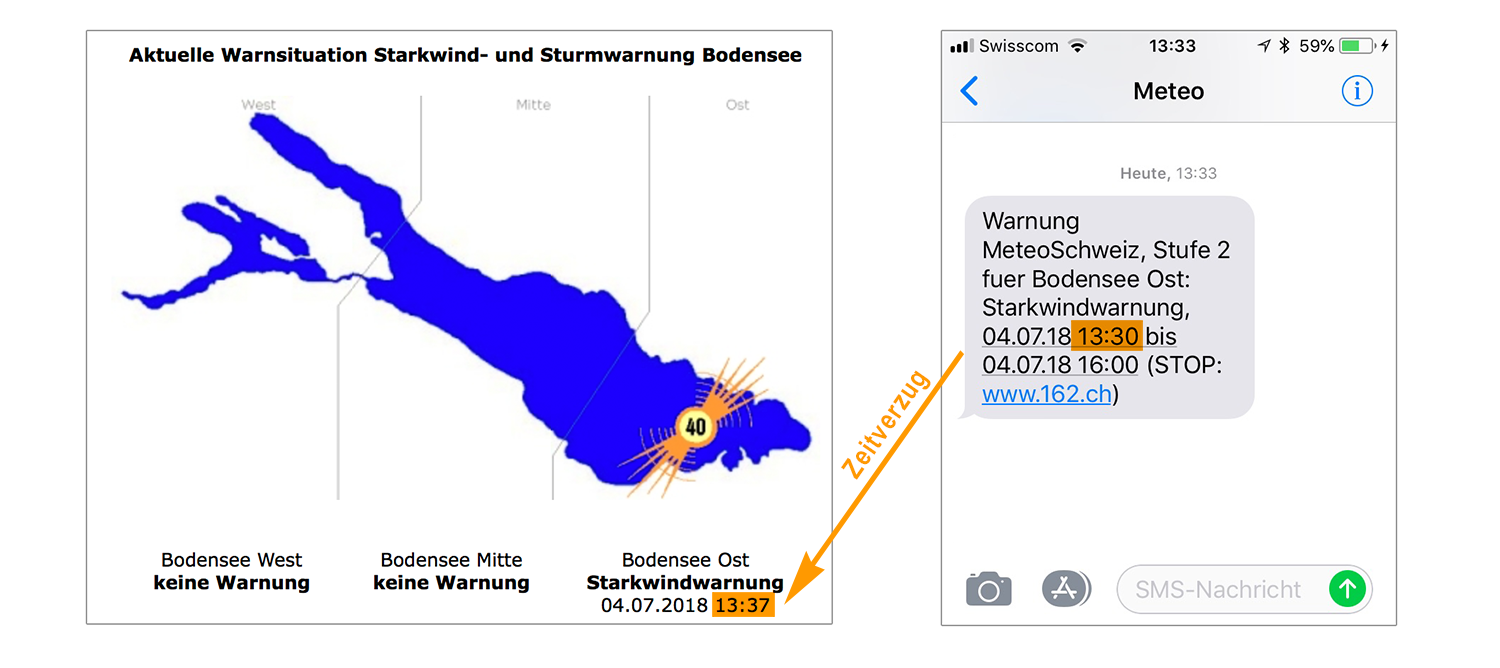
\includegraphics[width=\textwidth-2\fboxsep-2\fboxrule]{img/sturmZeit}}
	\caption[Zeitverzug zwischen Sturmwarnmeldung und Anzeige]{Zeitverzug zwischen der Warnmeldung von Meteoschweiz und dem Einschalten der Warnleuchten durch die Kantonale Notrufzentrale (KNZ) in Frauenfeld}
	\label{img:sturmZeit}
\end{figure}


\subsubsection{Eigener Sturmwarndienst mit Hilfe der Messwerte}
% Problem 2: Öffnungszeiten -> keine Warnung in der Nacht
Der Sturmwarndienst, wie in Abschnitt \ref{subsec:sturmwarnung} beschrieben, ist kein 24h-Service. Der Dienst ist nur tagsüber aktiv zu den aufgelisteten Warnzeiten~\cite{kapoStwrn}:

\begin{description*}
  \item[Sommer:] 1. April - 31. Oktober: 06:00 - 22:00 Uhr
  \item[Winter: ] 1. November - 31. März: 07:00 - 20:00 Uhr
\end{description*}

\noindent
% Problem 3: rechtliche Verbindlichkeit der Sturmwarnung -> Zuverlässigkeit der anzeigen
Es liegt nahe, auf Grund der eigenen Windmessdaten eine Sturmwarnung anzuzeigen bzw. einen Benachrichtungsservice, wie in Kapitel \ref{notifications} beschrieben, anzubieten. In der Bodensee-Schifffahrts-Ordnung (BSO) Art. 6.13, steht jedoch:

\begin{quote}
\flqq Bereits bei Starkwind- und Sturmwarnung muss der Schiffsführer die durch die Umstände gebotenen Massnahmen treffen.\frqq
\end{quote}

\noindent
 Da die Sturmwarnung auf dem Bodensee gesetzliche Pflichten mit sich bringt, wurde entschieden, nur die offiziellen Daten anzuzeigen und keine anderweitigen Sturmwarnungen.

% Meteoschweiz bietet zudem auf ihrer  \href{https://www.meteoschweiz.admin.ch/home/service-und-publikationen/beratung-und-service/meteoschweiz-app.html}{MeteoSchweiz-App} die Möglichkeit von Push-Nachrichten bei Windwarnungen.



%-> Meteoschweiz schickt in der Nacht keine SMS????? bzw. erstellt keine JSON????

% ins Kapitel API bzw. Cronjobs übernehmen
%Der Status der drei Teilabschnitte wird dann mintütlich in die Datenbank geschrieben. So kann der aktuelle Stand normal über die API abgefragt werden.

% nur im Vortrag erwähnen
% DAs JSON von Meteoschweiz kann leider nicht verwendet werden, da dessen URL bei jedem Update wechselt. Der genaue Pfad lässt sich nicht vorhersagen. Auf Grund des Zeitstempels lässt sich erahnen, dass es keine automatische Verbindung zwischen Meteoschweiz und den Sturmwarnleuchten am Bodensee gibt. Auf der Meteoschweiz-Seite ist z.B. der Zeitstempel 12:00 und auf der kttg.ch Seite 12:07. Wahrscheinlich erfolgt die Aktivierung manuell. Dies würde die Zeitdifferenz erklären.
% -> Foto Zeitstempel Meteoschweiz und kttg.ch
% Meteoschweiz leitet die Sturmwarnung an die Kantonspolizei Thurgau weiter. Diese schaltet die Sturmwarnung über eine eigne Software ein.


%% ############################################################################
%% Unterkapitel
%% ############################################################################
\subsection{Darstellung der historischen Daten}
Die historischen Daten der Wetterstation sollen öffentlich über die Website zugänglich sein. Die Darstellung soll möglichst interaktiv gestaltet sein und ein aussagekräftiges Bild des Wetterverhaltens aufzeigen. Bereits bei der alten Wetterstation wurden Daten gespeichert. Zudem liegt ein Excel-File vor mit den Pegeldaten der letzten 50 Jahre, welche ebenfalls auf der Webseite verfügbar sein sollen. Es gibt somit drei Grundlagen für die historischen Daten:

\begin{itemize*}
\item Historische Daten der neuen Wetterstation (2015 bis heute)
\item Historische Daten der alten Wetterstation (2005 bis 2012)
\item Exceltabelle mit historischen Pegeldaten (1953 bis 2005 )
\end{itemize*}

\noindent
Diese Daten und deren Anzeige auf der Webseite werden im Folgenden erläutert.

\subsubsection{Historische Daten der neuen Wetterstation}
\label{kap:Tableau}
 \href{https://public.tableau.com/de-de/s/}{\emph{Tableau Public}} ist ein Daten-Visualisierungsprogramm, welches es ermöglicht, auf einfache Weise Diagramme zu erstellen, welche interaktiv vom Benutzer filterbar sind. Der Benutzer kann zum Beispiel den Betrachtungszeitraum selbst wählen, worauf sich die Grafiken automatisch der Auswahl anpassen.

\begin{figure}[h!]
	\centering
  \fbox{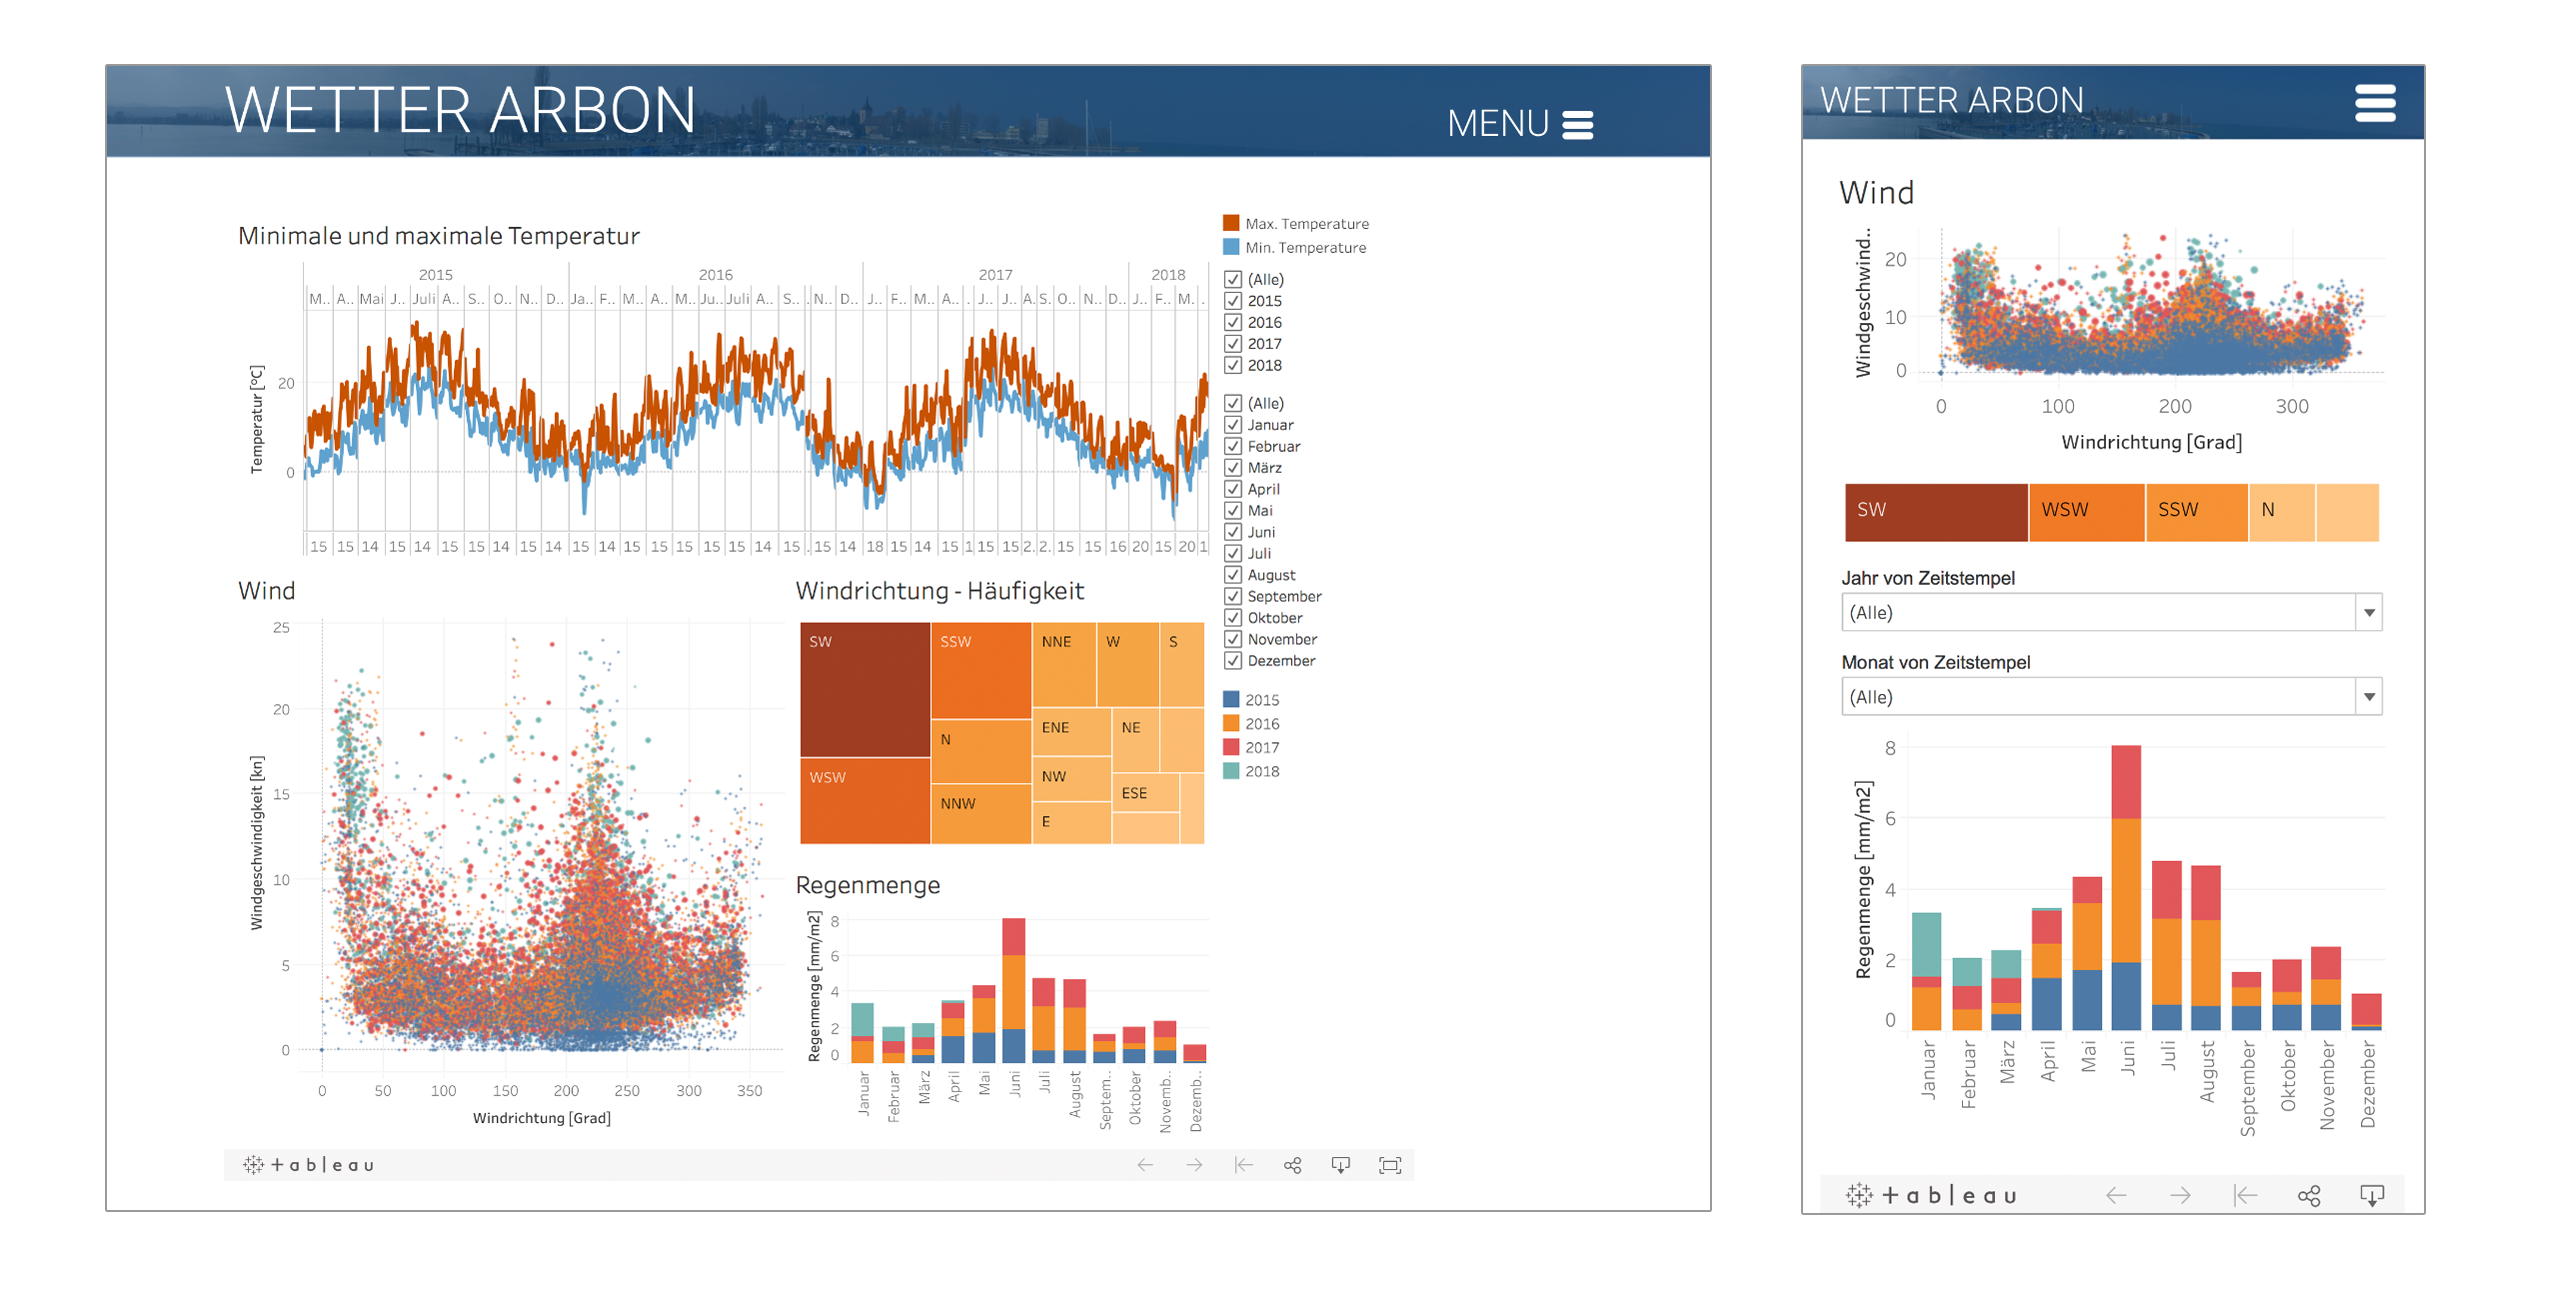
\includegraphics[width=\textwidth-2\fboxsep-2\fboxrule]{img/tableau}}
	\caption{Darstellung der historischen Daten (Desktop und Mobile)}
	\label{img:tableau}
\end{figure}


\noindent
\emph{Tableau Public} ist kostenlos mit der Einschränkung, dass sämtliche Visualisierungen öffentlich sind. In unserem Fall ist dies kein Problem, da die Visualisierungen sowieso veröffentlicht werden. Der Vorteil von Tableau ist, dass die Visualisierungen sehr einfach angepasst werden können, wenn z.B. neue Messgrössen hinzukommen. Tableau bietet zudem die Möglichkeit, Darstellungen für verschiedene Bildschirmgrössen anzulegen. Die Umsetzung ist in Abbildung\,\ref{img:tableau} dargestellt und unter dem Link \url{https://dev.wetter-arbon.ch/wetterhistorisch} abrufbar.

%Nachteil 2: Nicht responsive -> Workaround nötig
Neben den vielen Vorteilen hat Tableau Public auch ein paar Nachteile. Das Dashboard kann zwar frei gestaltet werden, ist aber nicht responsive d.h. es passt sich nicht der Bildschirmgrösse an. Das Problem wurde so gelöst, dass zwei verschiedene Dashboards erstellt wurden. Eines für die Anzeige auf einem grossen Bildschirm und eines für die Anzeige auf Mobiltelefonen (siehe Abbildung \ref{img:tableau}). Beim Aufruf der Webseite wird die Bildschirmgrösse abgefragt und das entsprechende Dashboard geladen wie in Listing \ref{lst:histViewport} dargestellt.

\vspace{3mm}
\begin{lstlisting}[label=lst:histViewport,caption=Auswahl des Dashboards anhand der Bildschirmgrösse, language=JavaScript, style=htmlcssjs]
(function () {
	var viewportWidth = $(window).width();
	if (viewportWidth > 767) {
		$('#area_3').load('application/php/tableauDesktop.php');}
	else {
		$('#area_3').load('application/php/tableauMobile.php');}
}());
\end{lstlisting}
\vspace{3mm}

% Nachteil 1: Keine direkte Verbindung zur Datenbank
\noindent
Ein weiterer Nachteil der Public-Version von Tableau ist, dass sie keinen Live-Zugriff auf die Datenbank ermöglicht. Die Daten müssen somit manuell periodisch auf den Tableau Public Server kopiert werden, damit sie im Dashboard verfügbar sind.

% Wenn mit dem Mauszeiger über einen Messpunkt gefahren wird, werden zusätzliche Informationen angezeigt.
% Für die Auswertung haben wir uns auf die Lufttemperatur, Sonnenstrahlung, Windrichtung und -geschwindigkeit sowie den Regen und Sonnenscheindauer konzentriert.


\subsubsection{Historische Daten der alten Wetterstation}
Um einen Überblick über die vorhandenen Messdaten der alten Wetterstation zu erhalten, wurden die Daten grafisch aufbereitet wie in Abbildung\,\ref{img:histAlt} dargestellt. Darin lassen sich diverse Messlücken erkennen wie zum Beispiel das komplette Jahr 2010 und 2012. Weiter sind zum Teil unplausible Grössenordnungen vorhanden wie zum Beispiel bei der Windgeschwindigkeit, wo die Werte im Bereich von 0 bis 1000 liegen und nicht klar ist, in welcher Einheit diese Daten vorliegen. Die Angaben der Wellenhöhe sind in einem sehr kleinen Bereich, sodass davon auszugehen ist, dass es sich um das Signalrauschen handelt und nicht um die effektiven Wellenhöhen. Alles in allem sind in diesen Daten nicht viele nützliche Informationen vorhanden. Es wurde deshalb beschlossen, auf der Webseite nur die historischen Daten der neuen Wetterstation d.h. ab 2015 anzuzeigen. Alleine die Pegeldaten werden verwendet und die historische Pegeldatenbank integriert, wie in Abschnitt \ref{subsec:pegelhistory} beschrieben.

\begin{figure}[h!]
	\centering
  \fbox{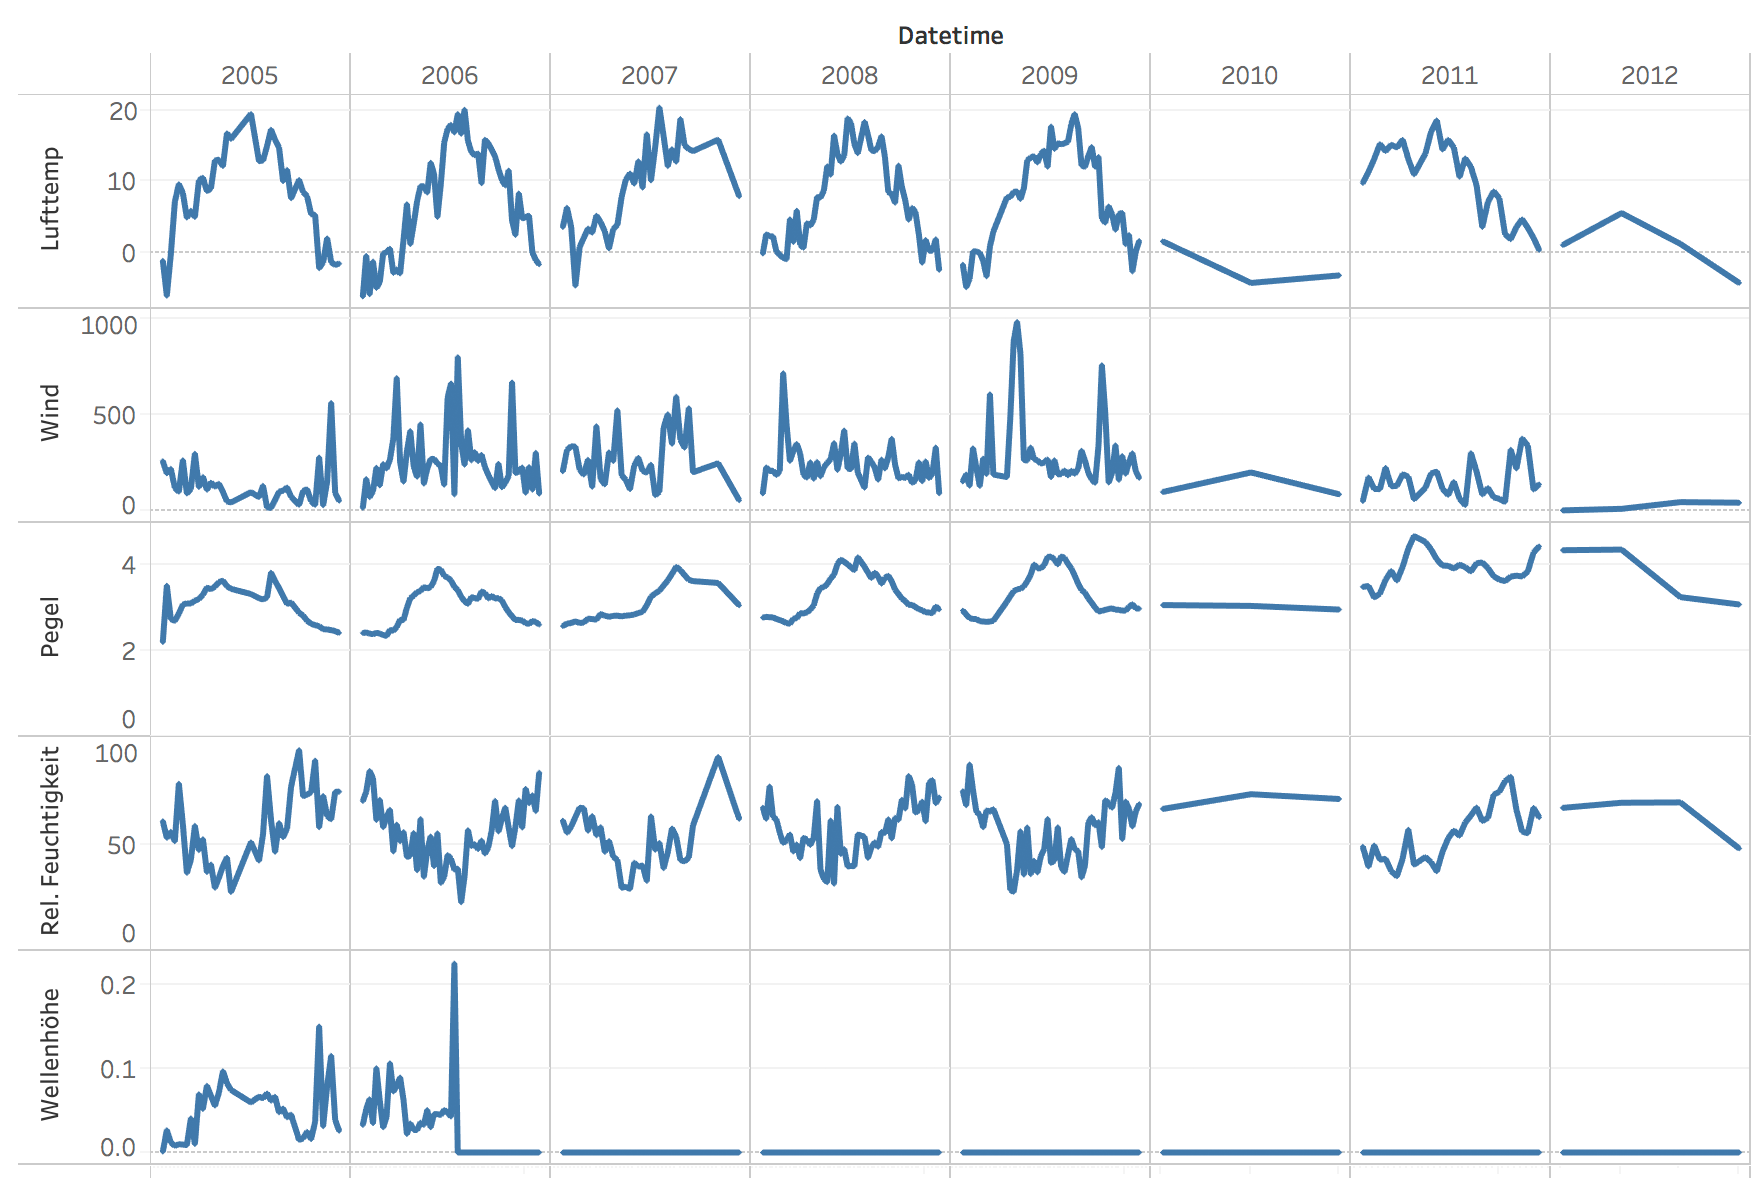
\includegraphics[width=\textwidth-2\fboxsep-2\fboxrule]{img/histAlt}}
	\caption{Übersicht über die gespeicherten Daten der alten Wetterstation}
	\label{img:histAlt}
\end{figure}



\subsubsection{Historische Pegeldaten}
\label{subsec:pegelhistory}
Auf der Webseite wird der Pegelverlauf der letzten Jahre grafisch dargestellt. Als Grundlage diente unter anderem ein Excel-File mit den Pegelständen von 1953 bis 2005. Von der alten Wetterstation liegen die Pegeldaten von 2005 bis 2009 vor und ab 2018 kommen die Messwerte der neuen Wetterstation dazu. Die Darstellung ist in Abbildung\,\ref{img:histPegel} ersichtlich. Sämtliche Datenquellen sind in einer gemeinsamen Tabelle in der Datenbank gespeichert. Die grafische Darstellung erfolgt wiederum mit Tableau, was die interaktiven Anzeige mit Filterung der Daten ermöglicht. Das Dashboard ist unter dem Link \url{https://dev.wetter-arbon.ch/pegelstand} erreichbar.

\begin{figure}[h!]
	\centering
  \fbox{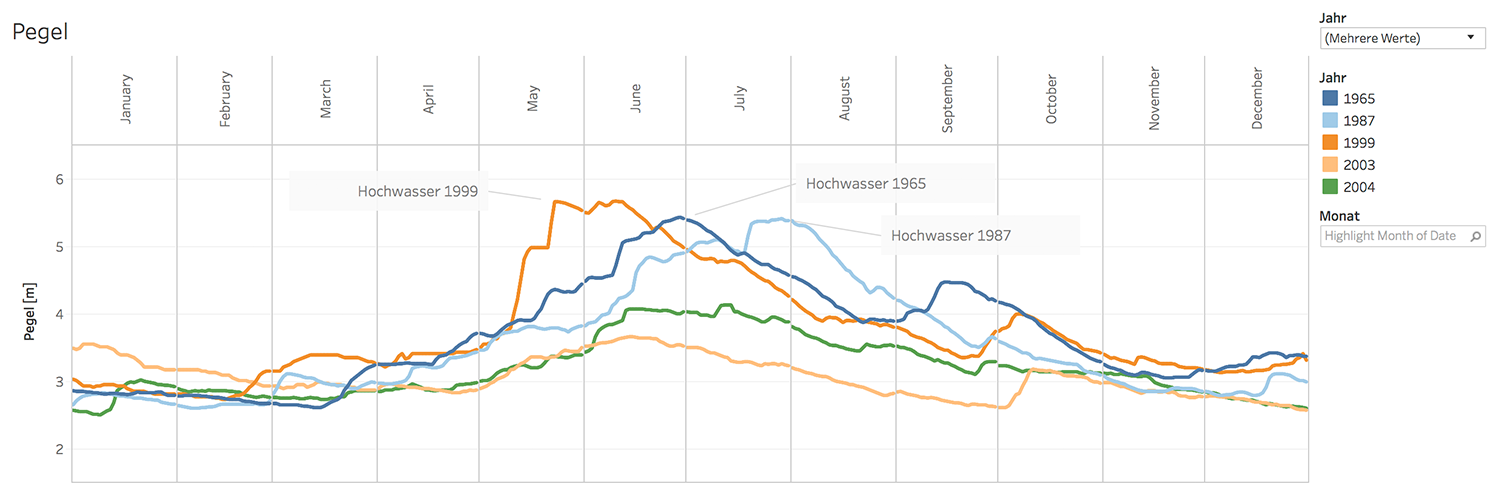
\includegraphics[width=\textwidth-2\fboxsep-2\fboxrule]{img/histPegel}}
	\caption{Darstellung der historischen Pegelmesswerte (gefiltert)}
	\label{img:histPegel}
\end{figure}



%% ############################################################################
%% Unterkapitel
%% ############################################################################
\subsection{Automatische Aktualisierung der Anzeigeelemente}
Die Wetterstation erzeugt jede Minute einen Datenbank-Eintrag mit den aktuellen Messwerten. Damit eine geöffnete Webseite immer auf dem aktuellen Stand ist, wird eine poll-Funktion verwendet, die selbständig alle 60\,Sekunden von der API die aktuellen Werte abfragt, wie in Listing\,\ref{lst:poll} verkürzt dargestellt. Sobald die JSON-Daten eingetroffen sind, wird die Funktion \emph{updateData} aufgerufen, die wiederum die Anzeigeelemente und Textfelder aktualisiert. Die gesamte Aktualisierung wird asynchron mittels AJAX durchgeführt. Die Seite wird dabei nicht neu geladen, nur die Anzeigewerte.

\begin{lstlisting}[label=lst:poll,caption=Automatische Aktualisierung der Werte, language=JavaScript, style=htmlcssjs]
(function poll() {
        $.get('https://api.wetter-arbon.ch/v1/')
          .done(function(response) {updateData(response);})
          .always(function() {setTimeout(poll, 60000); });
})();
function updateData(res){
        pressure_gauge.refresh(res.v1.data.pressure.value);
        $("#wassertemp1m") = res.v1.data.watertemperature1m.value;
        // usw.
}
\end{lstlisting}

\noindent
Damit die aktuellen Messwerte beim Aufbau der Seite zur Verfügung stehen, werden sie bereits beim Rendern der php-Seite von der API abgerufen und als JSON in der Variable \emph{initialValues} gespeichert (siehe Listing\,\ref{lst:initialValues}).

\begin{lstlisting}[label=lst:initialValues,caption=Übergabe der Initialisierungswerte durch php, language=JavaScript, style=htmlcssjs]
<script>
  var initialValues = JSON.parse('<?echo file_get_contents("https://api.wetter-arbon.ch/v1/");?>');
  document.getElementById("pegel").innerHTML = initialValues.v1.data.waterlevel.value;
  // usw.
</script>

\end{lstlisting}

%% ############################################################################
%% Unterkapitel
%% ############################################################################
\subsection{Barrierefreier Zugang}
Die Wetterstation und ihre Webseite ist eine Dienstleistung der Stadt Arbon. Sie gehört der Bevölkerung und soll deshalb möglichst für alle zugänglich sein. Sowohl die \emph{Web Content Accessibility Guidelines}~\cite{w3cwcag} des W3C-Konsortiums, als auch die deutsche \emph{Barrierefreie-Informationstechnik-Verordnung}~\cite{BITVde} bieten diverse Inputs, wie die Bedienbarkeit und somit Zugänglichkeit einer Webseite verbesserte werden kann. Von einer verbesserten Zugänglichkeit profitieren nicht nur Menschen mit Einschränkungen. Es geht darum, die Webseite so zu gestalten, dass sie möglichst für alle Benutzergruppen zugänglich ist. Eine von Microsoft beauftragte Studie~\cite{ForresterResearch2004E:Abilities} der \emph{Forrester Research Inc.} schätzt, dass über 60 Prozent aller Computernutzer von Barrierefreiheit profitieren können und gemäss Einschätzung des Verfassers des Buchs \emph{Interface Design}~\cite{ThesmannStephan2016ID:U} wird Barrierefreiheit bald Standard sein.

\noindent
Die aktuellen \emph{Web Content Accessibility Guidelines}~\cite{w3cwcag} fordern die Einhaltung von vier Designprinzipien, welche in gesamthaft zwölf Richtlinien genauer spezifiziert sind.

\begin{itemize*}
\item Designprinzip 1: wahrnehmbar
\item Designprinzip 2: bedienbar
\item Designprinzip 3: verständlich
\item Designprinzip 4: robust
\end{itemize*}

\noindent
Aus den Richtlinien wurden diejenigen Anforderungen ausgewählt, die auf die Webseite der Wetterstation anwendbar und die im Rahmen des CMS\footnote{CMS: Content Management System} umsetzbar sind. Alle relevanten Anforderungen und deren Umsetzung werden im Folgenden beschrieben.

\subsubsection{Wahrnehmbarkeit}
% Richtlinie 1.1
\href{https://www.w3.org/Translations/WCAG20-de/#text-equiv}{\textbf{Richtlinie 1.1}} fordert, dass für alle Nicht-Text-Inhalte eine Textalternative zur Verfügung steht. Auf der Webseite mit den aktuellen Messwerten gibt es drei Typen von Nicht-Text-Inhalten: Gauges, Icons und Graphen. Bei den Gauges und Graphen werden fertige Javascript-Bibliotheken verwendet. Diese stellen leider keine Möglichkeit zur Verfügung, einen Alternativtext hinzuzufügen. Für die Icons, welche als \emph{img} gekennzeichnet sind, wurde das \emph{alt}-Attribut ausgefüllt, wie in Listing \ref{lst:altImg} beispielhaft dargestellt.

\begin{lstlisting}[label=lst:altImg,caption=Alternativtext für Icons, language=HTML5, style=htmlcssjs]
<img src="img/wi-humidity.svg" alt="Icon eines Barometers">
\end{lstlisting}

\noindent
Wie die verwendeten javascript-Bibliotheken bietet auch Tableau, mit welchem die interaktive Darstellung der historischen Daten erfolgt, keine Möglichkeit, die Visualisierung als Text darzustellen. Das bedeutet, dass eine Reihe von Informationen auf dem gegenwärtigen technischen Stand noch nicht durch alternative Texte barrierefrei dargestellt werden können. \newline

% Richtlinie 1.3
\noindent
\href{https://www.w3.org/Translations/WCAG20-de/#text-equiv}{\textbf{Richtlinie 1.3}} fordert, dass die Struktur d.h. die Zusammenhänge und die Bedeutung einer Webseite unabhängig der Formatierung erhalten bleiben. Man spricht hier auch von \emph{semantischem} Web. Auf der Webseite wurde eine hierarchische Struktur implementiert, siehe Abbildung \ref{img:semWeb}. Die Hierarchiestufe wird einerseits erkennbar durch die Stufe der Überschriften (h1...h3) und andererseits durch die Bezeichnung der verschiedenen Inhaltsblöcke. Auf der Webseite sind zwei Hauptblöcke erkennbar, sogenannte \emph{Sektionen}. Eine Sektion beinhaltet die aktuellen Messwerte und die andere die Messdatenverläufe. Eine \href{https://www.w3.org/TR/2011/WD-html5-20110525/sections.html#the-section-element}{\emph{Sektion}} ist eine thematische Gruppierung von Elementen. Innerhalb der Sektion gibt es mehrere \href{https://www.w3.org/TR/2011/WD-html5-20110525/sections.html#the-article-element}{\emph{Artikel}}, welche einen unabhängigen Informationsblock darstellen.
\newpage

\begin{figure}[h!]
	\centering
  \fbox{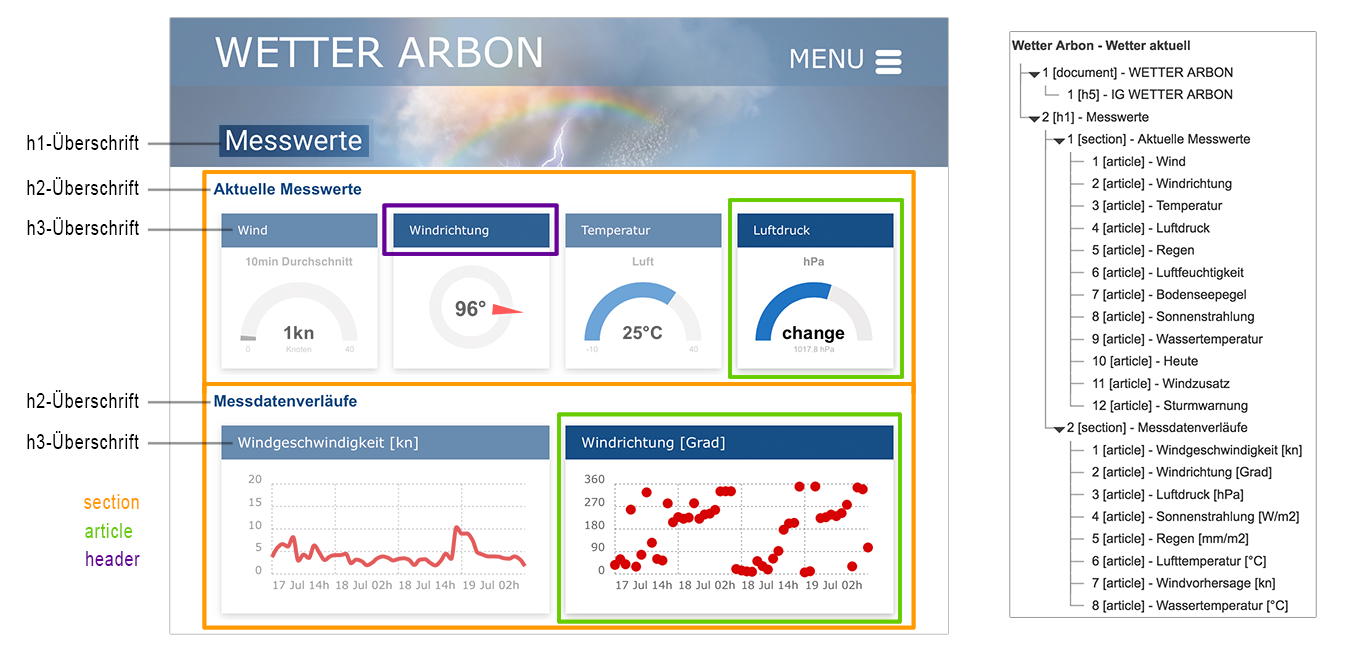
\includegraphics[width=\textwidth-2\fboxsep-2\fboxrule]{img/semWeb}}
	%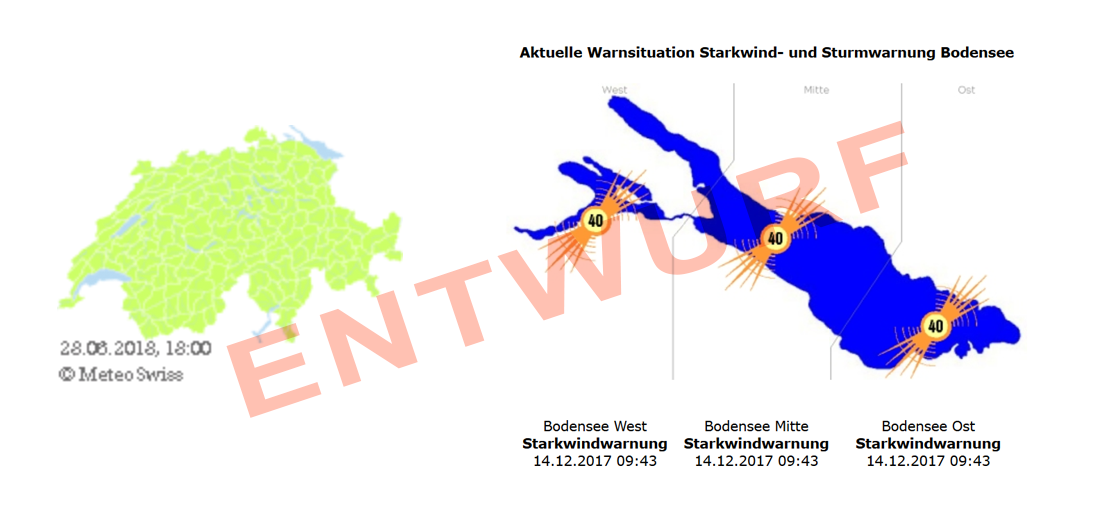
\includegraphics[width=1\linewidth]{img/sturm}
	\caption{Umsetzung der Anforderung bezüglich Semantischem Web}
	\label{img:semWeb}
\end{figure}

% Richtlinie 1.4
\noindent
\href{https://www.w3.org/Translations/WCAG20-de/#visual-audio-contrast}{\textbf{Richtlinie 1.4}} fordert, dass die visuelle Darstellung von Text ein Kontrastverhältnis von mindestens 4,5:1 hat. Zudem muss es möglich sein die Textgrösse um bis zu 200 Prozent zu erhöhen, ohne dass dabei Inhalt oder Funktionalität verloren geht. Um diese Anforderung zu überprüfen, wurde das Firefox-Plugin \textit{tota11y}\footnote{\url{http://khan.github.io/tota11y/}} verwendet. Das Plugin ermöglicht es, auf einfache Weise zu überprüfen, ob die Webseite die Barrierefrei-Bediungungen erfüllt. Die Kontrastverhältnisse liegen gemäss diesem Tool zwischen 5.75 und 12.63 und erfüllen somit die Anforderung. Da die gesamte Webseite responsive ist, stellt die Vergrösserung auf 200\% kein Problem dar.


\subsubsection{Bedienbarkeit}
\href{https://www.w3.org/Translations/WCAG20-de/#keyboard-operation}{\textbf{Richtlinie 2.1}} fordert, dass alle Funktionen über eine Tastaturschnittstelle bedienbar sind und dass die Tastaturfokusanzeige sichtbar ist.
Da es sich bei der Webseite der Wetterstation primär um eine Anzeige handelt, ist dieses Anforderung nur für das Eingabeformular des Benachrichtigungsservice (siehe Kapitel\,\ref{notifications}) relevant. Das Eingabeformular ist problemlos mittels Tastatur bedienbar.\newline

\noindent
\href{https://www.w3.org/Translations/WCAG20-de/#navigation-mechanisms}{\textbf{Richtlinie 2.4}} fordert, dass Webseiten einen zweckbeschreibenden Titel aufweisen und dass Zwischentitel den Inhalt und Zweck des entsprechenden Blocks beschreiben. Wie in Abbildung \ref{img:semWeb} dargestellt, besitzt die Webseite sowohl einen Seitentitel, als auch Zwischentitel.

\newpage
\subsubsection{Verständlichkeit}
\href{https://www.w3.org/Translations/WCAG20-de/#minimize-error}{\textbf{Richtlinie 3.3}} fordert, dass Eingabefehler automatisch erkannt und dem Benutzer angezeigt werden. Zudem sind Korrekturvorschläge anzuzeigen. Diese Anforderung betrifft insbesondere das Formular des Benachrichtigungsservices, welches in Kapitel\,\ref{notifications} beschrieben wird. Diese Anforderung wird erfüllt, wie in Abbildung \ref{img:notificationFE} links auf Seite \pageref{img:notificationFE} dargestellt.


\subsubsection{Robustheit}
\href{https://www.w3.org/Translations/WCAG20-de/#ensure-compat}{\textbf{Richtlinie 4.1}} fordert, dass Inhalte, die mit Hilfe von Markup-Sprachen implementiert wurden,  vollständige Start- und End-Tags haben. Es sind keine doppelten Attribute vorhanden und alle IDs sind eindeutig. Diese Anforderung wurde ebenfalls vollständig umgesetzt. Beispielhaft ist dies in Listing \ref{lst:gaugeHTML} auf Seite \pageref{lst:gaugeHTML} ersichtlich.
